\documentclass[tikz, border = 0.1cm]{article}
\usepackage{tikz}
\usetikzlibrary{bayesnet}
\usepackage{amsmath, amsthm, amssymb, amsfonts}
\tikzset{>=latex}
\usepackage{filecontents}
\usepackage{placeins}
% if you need to pass options to natbib, use, e.g.:
    \PassOptionsToPackage{numbers, compress}{natbib}
% before loading neurips_2024


% ready for submission
\usepackage{neurips_2024}


% to compile a preprint version, e.g., for submission to arXiv, add add the
% [preprint] option:
%     \usepackage[preprint]{neurips_2024}


% to compile a camera-ready version, add the [final] option, e.g.:
%     \usepackage[final]{neurips_2024}


% to avoid loading the natbib package, add option nonatbib:
% \usepackage[nonatbib]{neurips_2024}
\usepackage{natbib} % has a nice set of citation styles and commands
\bibliographystyle{plainnat}
\renewcommand{\bibsection}{\section*{References}}

\usepackage[utf8]{inputenc} % allow utf-8 input
\usepackage[T1]{fontenc}    % use 8-bit T1 fonts
\usepackage{hyperref}       % hyperlinks
\usepackage{url}            % simple URL typesetting
\usepackage{booktabs}       % professional-quality tables
\usepackage{amsfonts}       % blackboard math symbols
\usepackage{nicefrac}       % compact symbols for 1/2, etc.
\usepackage{microtype}      % microtypography
\usepackage{xcolor}         % colors

%\usepackage{enumitem}
\usepackage[textsize=tiny]{todonotes}

% Added by Lokesh

%%%%%%%%%%%%%For putting tables side-by-side%%%%%%%%%
\usepackage{float}
\usepackage{caption}

\usepackage{geometry}
\usepackage{array}
\newcolumntype{C}[1]{p{#1}}
\usepackage{icomma}
\usepackage{ragged2e}
\usepackage{wrapfig,lipsum,booktabs}
\RequirePackage[inline,shortlabels]{enumitem}
\usepackage{algorithmic}
\usepackage{algorithm}
%%%%%%%%%%%%%%%%%%%%%%%%%%%%%%%%%%%%%%%%%%%%%%%%%%%%%

\usepackage{graphicx}
\usepackage{subcaption}
\usepackage{booktabs} 
\usepackage{xcolor,colortbl}
\definecolor{green}{rgb}{0.8,1,0.8}
\definecolor{yellow}{rgb}{1,1,0.87}
\definecolor{cyan}{rgb}{0.0, 1.0, 1.0}
\newcommand{\first}[1]{{\cellcolor{green} #1}}
\newcommand{\second}[1]{{\cellcolor{yellow} #1}}
\newcommand{\third}[1]{{\cellcolor{cyan!50} #1}}

\usepackage{subdef}
\usepackage{multirow}
\newcommand{\yhat}{\widehat{y}}
\newcommand{\indep}{\rotatebox[origin=c]{90}{$\models$}}

% \usepackage{algpseudocode}
% \usepackage{algorithm}
\usepackage{hyperref}


\usepackage[subtle]{savetrees}

% For bayesnets
\usepackage{tikz}
\usetikzlibrary{bayesnet}
\usetikzlibrary{arrows}
\usepackage{color}
\usepackage{graphicx}
\usepackage{caption}
\usepackage{subcaption}
\usetikzlibrary{backgrounds}

\usepackage{titlesec}

% minimize spacing
% \titlespacing\section{0pt}{1pt plus 0pt minus 1pt}{1pt plus 0pt minus 1pt}
\titlespacing\subsection{0pt}{0pt plus 1pt minus 1pt}{0pt plus 1pt minus 1pt}
\titlespacing\subsubsection{0pt}{0pt plus 1pt minus 1pt}{0pt plus 1pt minus 1pt}
\titlespacing{\lemma}{0pt}{0pt plus 1pt minus 1pt}{0pt plus 1pt minus 1pt}

\newcommand{\xhdr}[1]{\vspace{1.5mm}\noindent{\bf #1.}}

\newcommand{\recourse}{recourse}
\newcommand{\bij}{\beta^i _j}
\newcommand{\bpij}{\widetilde{\beta}^i _j}
\newcommand{\net}{{\textsc{nn}}}
\newcommand{\gen}{\mathcal{Z}}
\newcommand{\genS}{\mathcal{Z}_S}
\newcommand{\geninv}{\gen^{-1}}
\newcommand{\genSinv}{\genS^{-1}}
\newcommand{\betabp}{\betab'}

\newcommand{\betaij}{\betab_{ij}}
\newcommand{\q}{q}
\newcommand{\betair}{\betab_{ir}}
\newcommand{\xij}{\xb_{ij}}
\newcommand{\xir}{\xb_{ir}}
% \newcommand{\xi}{x_{i}}
\newcommand{\yi}{y_{i}}
\newcommand{\betai}{\betab_i}
\newcommand{\sij}{S_{ij}}
\newcommand{\xit}{\xb_{it}}
\newcommand{\rhoij}{\rho_{ij}}
\newcommand{\betait}{\betab_{it}}
\newcommand{\y}{y}
\newcommand{\betaprior}{\betab^{prior}}
\newcommand{\gd}{gd}
\newcommand{\betaiprior}{\betab_i^{prior}}
\newcommand{\thhatnet}{f_{\widehat{\theta}}}
\newcommand{\genp}{\Pr_{\text{gen}}}
\newcommand{\rhohat}{\widehat{\rho}}

\newcommand{\RbetaInv}[1]{\Rbeta{#1}^{-1}}
\newcommand{\Sbeta}[1]{\mat{S}_{#1}}
\newcommand{\SbetaInv}[1]{\Sbeta{#1}^{-1}}
\newcommand{\wbeta}[1]{w_{#1}}
\newcommand{\wbetas}[1]{w_{#1}^S}

\newcommand{\thnet}{{f_\theta}}
\newcommand{\trnD}{D_{\text{trn}}}
\newcommand{\tstD}{D_{\text{tst}}}
\newcommand{\synD}{D_{\text{syn}}}
\newcommand{\Zspace}{\mathcal{Z}}
\newcommand{\synz}{\Tilde{z}}
\newcommand{\Tspace}{\mathcal{T}}
\newcommand{\xspace}{\mathcal{X}}
\newcommand{\yspace}{\mathcal{Y}}
\newcommand{\xSspace}{\mathcal{X}_S}
\newcommand{\Lspace}{\mathcal{L}}
\renewcommand{\yspace}{\mathcal{Y}}
\newcommand{\lhat}{\widehat{l}}
\newcommand{\zextS}{\Phi_S}
\newcommand{\zextR}{\Phi_R}
\newcommand{\mat}[1]{\boldsymbol{#1}}
\newcommand{\recmdl}{g_\phi}
\newcommand{\realwb}{w}
\newcommand{\realwbhat}{\widehat{w}}
\newcommand{\synwb}{w^S}
\newcommand{\synwbhat}{\widehat{w}^S}
\newcommand{\naivew}{w_{t}^D}
\newcommand{\directw}{w_{t}^D}
\newcommand{\jointw}{w_{t}^J}
\newcommand{\factualw}{w_{t}^F}
\newcommand{\jointR}{\widehat{\mat{R}}_{\betab}^{-1}}
\newcommand{\jointS}{\mat{S}_{\betab}^{-1}}

\newcommand{\Rbeta}[1]{\mat{R}_{#1}}



\newcommand{\jointwp}{w_{t}^J}
\newcommand{\jointRp}{\mat{R}_{t}^{-1}}
\newcommand{\jointSp}{\mat{S}_{t}^{-1}}
\newcommand{\realmu}{\mu}
\newcommand{\synmu}{\mu^S}
\newcommand{\realmuhat}{\widehat{\mu}}
\newcommand{\synmuhat}{\widehat{\mu}^S}
\newcommand{\synmuTilde}{\widetilde{\mu}^S}


\newcommand{\ITEx}{\tau_X}
\newcommand{\ITExhat}{\widehat{\ITEx}}
\newcommand{\ITExSyn}{\ITEx^S}
\newcommand{\tauhat}{\widehat{\tau}}
\newcommand{\syntau}{\tau^S}
\newcommand{\syntauhat}{\widehat{\tau}^S}
\newcommand{\syntauTilde}{\widetilde{\tau}^S}

\newcommand{\gapRR}{\lambda_{R}}
\newcommand{\gapRS}{\lambda_{RS}}
\newcommand{\gapwR}{\lambda_{w}}
\newcommand{\gapwS}{\lambda_{wRS}}

\newcommand{\noise}{\mathcal{N}(0,1)}
\newcommand{\cX}{\mathcal{X}}
\newcommand{\cK}{\mathcal{K}}

\newcommand{\nind}{\not\!\perp\!\!\!\perp}

\newcommand{\betarv}{\mathfrak{B}}
\newcommand{\our}{\textit{SimPONet}}


\newcommand{\RInv}{f}
\newcommand{\RzInv}{f_0}
\newcommand{\RoInv}{f_1}
\newcommand{\RInvhat}{\widehat{f}}
\newcommand{\RzInvhat}{\widehat{f}_0}
\newcommand{\RoInvhat}{\widehat{f}_1}
\newcommand{\R}{g}
\newcommand{\Rz}{g_0}
\newcommand{\Ro}{g_1}
\newcommand{\SInv}{f^S}
\newcommand{\SInvTilde}{\widetilde{f}^S}
\newcommand{\SInvCont}{\SInvTilde}
\newcommand{\SInvhat}{\widehat{f}^S}
\newcommand{\SzInv}{f^S_0}
\newcommand{\SoInv}{f^S_1}
\renewcommand{\S}{g^S}
\newcommand{\Sz}{g^S_0}
\newcommand{\So}{g^S_1}
\newcommand{\Shat}{\widehat{g}^S}
\newcommand{\Szhat}{\widehat{g}^S_0}
\newcommand{\Sohat}{\widehat{g}^S_1}
\newcommand{\LRfct}{\lambda_{\text{fct}}}
\newcommand{\LSfct}{\lambda^S_{\text{fct}}}
\newcommand{\LScf}{\lambda^S_{\text{cf}}}
\newcommand{\Lphi}{\lambda_{\RInv}}
\newcommand{\Ltau}{\lambda_{\tau}}
\newcommand{\ErrITE}{\mathcal{E}_{\text{CATE}}}
\newcommand{\ErrF}{\mathcal{E}_F}
\newcommand{\ErrCF}{\mathcal{E}_{CF}}
\newcommand{\ErrCFR}{\mathcal{E}_{CF}^R}
\newcommand{\ipm}[1]{\textsc{IPM}_{#1}}
\newcommand{\ipmg}{\ipm{G}}
\newcommand{\distR}{\texttt{dist}(\realmu \circ \RInv, \realmu \circ \SInv)}
\newcommand{\distmu}{\texttt{dist}(\realmu \circ \SInv, \synmu \circ \SInv)}
\newcommand{\distcont}{\texttt{dist}(\SInv, \SInvCont)}

\newcommand{\simonly}{SimOnly}
\newcommand{\realonly}{RealOnly}
\newcommand{\muonly}{$\text{Real}_\mu\text{Sim}_f$} %{$\mu$Only}
\newcommand{\epsf}{\epsilon_{\RInv}}
\newcommand{\delf}{\delta_{\RInv}}
\newcommand{\epsmu}{\epsilon_{\realmu}}
\newcommand{\delmu}{\delta_{\realmu}}



%%%%%%%%%%%%%%%%%%%%%%%
% Color Block
%%%%%%%%%%%%%%%%%%%%%%%
\usepackage{xcolor} 
\usepackage{tikz} 
\usepackage{tcolorbox}
\tcbuselibrary{skins,breakable}
\usetikzlibrary{shadings,shadows}
\newenvironment{gblock}[1]{%
\tcolorbox[beamer,%
noparskip,breakable,
colback=LightGreen,colframe=DarkGreen,%
colbacklower=LimeGreen!75!LightGreen,%
title=#1]}%
{\endtcolorbox}


%%%%%%%%%%%%%%%%%%%%%%%%%%%%%%%%%%%%%%%%%%%%%
% Added by Lokesh
%%%%%%%%%%%%%%%%%%%%%%%%%%%%%%%%%%%%%%%%%%%%%

\usetikzlibrary{shapes, arrows, calc, arrows.meta, fit, positioning} % these are the parameters passed to the library to create the node graphs  
\tikzset{  
    -Latex,auto,node distance =1.5 cm and 1.3 cm, thick,% node distance is the distance between one node to other, where 1.5cm is the length of the edge between the nodes  
    state/.style ={ellipse, draw, minimum width = 0.9 cm}, % the minimum width is the width of the ellipse, which is the size of the shape of vertex in the node graph  
    point/.style = {circle, draw, inner sep=0.18cm, fill, node contents={}},  
    bidirected/.style={Latex-Latex,dashed}, % it is the edge having two directions  
    el/.style = {inner sep=2.5pt, align=right, sloped}  
}  
\usepackage{multirow}

\title{Leveraging a Simulator to Estimate Treatment Effects from Post-Treatment Covariates}


% The \author macro works with any number of authors. There are two commands
% used to separate the names and addresses of multiple authors: \And and \AND.
%
% Using \And between authors leaves it to LaTeX to determine where to break the
% lines. Using \AND forces a line break at that point. So, if LaTeX puts 3 of 4
% authors names on the first line, and the last on the second line, try using
% \AND instead of \And before the third author name.


\author{%
  David S.~Hippocampus\thanks{Use footnote for providing further information
    about author (webpage, alternative address)---\emph{not} for acknowledging
    funding agencies.} \\
  Department of Computer Science\\
  Cranberry-Lemon University\\
  Pittsburgh, PA 15213 \\
  \texttt{hippo@cs.cranberry-lemon.edu} \\
  % examples of more authors
  % \And
  % Coauthor \\
  % Affiliation \\
  % Address \\
  % \texttt{email} \\
  % \AND
  % Coauthor \\
  % Affiliation \\
  % Address \\
  % \texttt{email} \\
  % \And
  % Coauthor \\
  % Affiliation \\
  % Address \\
  % \texttt{email} \\
  % \And
  % Coauthor \\
  % Affiliation \\
  % Address \\
  % \texttt{email} \\
}


\begin{document}


\maketitle

\vspace{-5mm}
\begin{abstract}
\vspace{-3mm}
Treatment effect estimation involves assessing the impact of different treatments on individual outcomes. Current methods rely on observational datasets where covariates are gathered before treatments and outcomes are observed afterward. However, real-world scenarios often deviate from this protocol, leading to both covariate and outcome observed 
% collection simultaneously 
post-treatment. We first establish that this deviation renders treatment effects unidentifiable, necessitating additional assumptions for estimation. We propose \our, which unlike prior methods that assume counterfactual supervision in the training datasets, assumes the availability of a simulator that generates related synthetic counterfactual data. This allows recovery of latent pre-treatment covariates 
% upto a diffeomorphic transformation 
which aid in treatment effect identification. The accuracy of such estimates hinges on the quality of the simulator, and we conduct theoretical analyses to establish generalization bounds that assess the CATE error based on the distributional discrepancies between real and synthetic data. In a linear setting, we analytically derive the CATE error, demonstrating the limitations of several baseline methods. Our empirical validation on synthetic and semi-synthetic real world datasets further reinforces \our's effectiveness in precise treatment effect estimation from post-treatment data.
\end{abstract}



\section{Introduction} \label{sec:intro}
% \begin{gblock}{On the writing}
%     \begin{enumerate}
%         \item Other than post-T bias
%         \item Realistic Example for post-T
%         \item Layout of different models.
%         \item Neurips? I am for it!
%         \item Research Qns for the Experiments (assuming just IHDP, Linear)
%     \end{enumerate}
% \end{gblock}
\vspace{-0.1in}
\begin{wrapfigure}{r}{0.35\textwidth}
  \vspace{-0.7cm}
  \begin{center}
    {\resizebox{0.35\textwidth}{!}{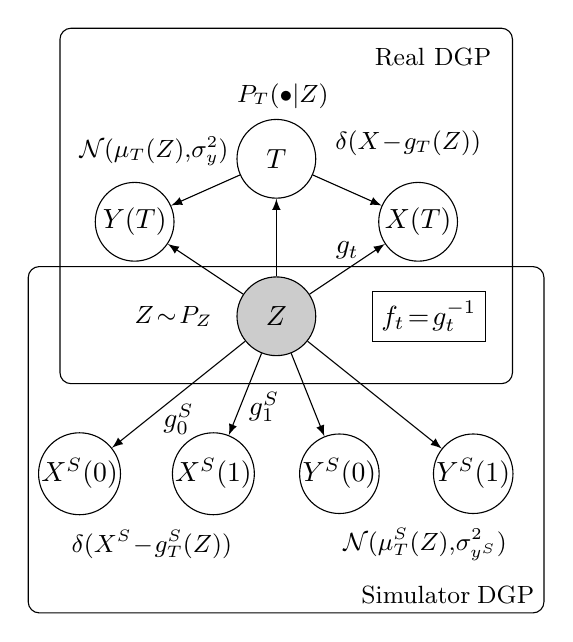
\begin{tikzpicture}

    \node[circle, draw = black, fill = gray!40, inner sep = 0pt, minimum size = 1cm] (z) at (0, 0) {{$Z$}};
    \node[circle, draw = black, inner sep = 0pt, minimum size = 1cm] (t) at (0, 2) {{$T$}};
    \node[circle, draw = black, inner sep = 0pt, minimum size = 1cm] (yt) at (-1.8, 1.2) {{$Y(T)$}};
    \node[circle, draw = black, inner sep = 0pt, minimum size = 1cm] (xt) at (1.8, 1.2) {{$X(T)$}};
    \node[circle, draw = black, inner sep = 0pt, minimum size = 1cm] (xs0) at (-2.5, -2) {{$X^S(0)$}};
    \node[circle, draw = black, inner sep = 0pt, minimum size = 1cm] (xs1) at (-0.8, -2) {{$X^S(1)$}};
    \node[circle, draw = black, inner sep = 0pt, minimum size = 1cm] (ys0) at (0.8, -2) {{$Y^S(0)$}};
    \node[circle, draw = black, inner sep = 0pt, minimum size = 0.55cm] (ys1) at (2.5, -2) {{$Y^S(1)$}};
    
    \foreach \n in {t, yt, ys0, ys1}{\path [draw, ->] (z) edge (\n);}
    \path [draw, ->] (z) edge node[midway, above] {$g_t$} (xt);
    \path [draw, ->] (z) edge node[midway, below] {$g_0^S$} (xs0);
    \path [draw, ->] (z) edge node[pos=0.35, below, xshift=5pt] {$g_1^S$} (xs1);
    \path [draw, ->] (t) edge (yt);
    \path [draw, ->] (t) edge (xt);
     \node[draw, rectangle, right=20pt of z] {$f_t = g_t^{-1}$};
    
    \node[text width=1.5cm] (realdis) at (2, 3.3) {\small{Real DGP}};
    
    \node[text width = 1.2cm] (pz) at (-1.2, 0.) {\small{$Z \sim P_Z$}};
    \node[text width = 1cm] (pyt) at (-2, 2.1) {\small{$\mathcal{N}(\realmu_T(Z), \sigma_y^2)$}};
    \node[text width = 2cm] (pt) at (0.5, 2.8) {\small{$P_T(\bullet|Z)$}};
    \node[text width = 1.9cm] (pxt) at (1.7, 2.2) {\small{$\delta(X - \R_T(Z))$}};
    
    \node[text width = 3cm] (pxs) at (-1.1, -2.9) {\small{$ \delta(X^S - \S_T(Z))$}};
    \node[text width = 2.3cm] (pys) at (2, -2.9) {\small{$\mathcal{N}(\realmu^S_T(Z), \sigma_{y^S}^2)$}};
    
    \plate[] {plate1} {(z) (yt) (t) (xt) (pz) (pyt) (pt) (pxt) (realdis)} {};
    \plate[] {plate1} {(z) (ys0) (ys1) (xs0) (xs1) (pxs) (pys)} {\small{Simulator DGP}};

\end{tikzpicture}}}
  \end{center}
  \caption{The Data Generating process for Real and Simulator.\label{fig:our_DGP}}
  \vspace{-0.8cm}
\end{wrapfigure}
Many applications require estimating the difference in outcome as a result of a change in treatment. For example, in healthcare, we want to estimate the change in a patient's response as we prescribe different drugs. %In economics, we want to estimate the difference in social metrics as we implement alternate policies, etc. 
Randomized Control Trials are often expensive, and with the easy availability of observational data, there is extensive interest in harnessing observational data for these estimates. Existing works~\cite{xlearner,rlearner,CurthS23,cfrnet,vcnet,Tarnet, chauhan2023adversarial, inducbias, overlapping_rep, dragonnet,matching_survey} assume that the covariates are observed pre-treatment and the outcome post-treatment, whereas we are interested in the setting where both are observed post-treatment. %and the main challenge they try to address is estimating treatment effect when a given individual is subject to only one treatment.
%

In many real-life applications both covariates and outcomes are observed post-treatment.
%Conventional methods approach this problem through A/B testing or via Randomized Control Trials.  In both these approaches, we first collect a group of individuals that participate in a trial. We record different covariates associated with the individuals and then assign treatments to them arbitrarily. Finally, we measure the outcomes and derive statistical estimates that assess the impact of the treatments. However, in many domains, such trials are not always possible because they are either unethical or raise cost concerns. In response, research has been done to assess the effects from observational datasets where we do not have control over treatment assignments. 
% One consequence of this is that the dataset exhibits confounding where the observed treatments depend on covariates. For example, in medicine, aged patients often exhibit a higher propensity of being assigned treatments with heavy dosages. Such confounding issues are known to hurt the effect estimates and a lot of methods are proposed in prior art to account for them. 
% However, one common theme across all prior-art is that they assume that the covariates are recorded pre-treatment, i.e., {\em before} an individual is given the treatment.
% , and most of the Prior-art primarily focuses on mitigating confounding effects within the dataset. 
% Various techniques, such as \todo{cite heavily} meta-learners, representation learners, matching, and weighting, have been proposed for this purpose. 
%
% \todo[inline]{Need a compelling example}
%
%\textbf{Post-Treatment covariates are common: }  
%Existing methods typically rely on the assumption that covariates are collected before treatment and outcomes are observed afterward. However, in many real-life contexts, covariates and outcomes are often collected simultaneously after treatment, posing challenges for conventional methods such as meta-learners~\cite{xlearner,rlearner,CurthS23}, matching methods~\cite{matching_survey, prop_score_matching, coarsened_exact_matching, perfect_match, deepmatch}, generative models such as GANs~\cite{scigan,cevae}, and representation learners ~\cite{cfrnet,vcnet,Tarnet, chauhan2023adversarial, inducbias, overlapping_rep, dragonnet}. 
%Post-treatment covariates are common in various fields. 
For example, in economics ~\cite{policy_1, policy_2}, policy efficacy often needs to be assessed in settings where
%is usually assessed by comparing social metrics across treated and control groups. It is highly impractical to expect the same set of individuals to participate in the trial twice—first to provide covariates before and then to provide outcomes after policy implementation. Therefore, it is necessary to develop methods that work with 
both outcomes and covariates are available post-policy implementation. Similarly, in voluntary healthcare surveys only post-treatment data about patients may be available.  In medical imaging, an image may be observed under a given instrument setting (treatment), and it may be necessary to choose an alternative setting under which a downstream diagnosis (outcome) could improve. 
%like COVID-19 vaccination administration \cite{covid_postt}, patient covariates are collected post-vaccination to assess side effects.


We model the estimation of causal effects with observed post-treatment covariates and outcomes using a 
%
%\textbf{Our Data Generating Process (DGP):} We consider an observational dataset $\trnD$ containing samples from a real 
Data Generating Process (DGP) as outlined in the top panel of Figure \ref{fig:our_DGP} marked Real DGP. Here, \textit{latent} variables $Z$ influence treatment $T$, outcome $Y$, and covariates $X$. The latent nature of $Z$ impedes the identifiability of treatment effects solely given i.i.d samples $\trnD$ from the observed nodes.  
\todo[inline]{L: Lemma -- $\tau$ cannot be identified from observational dataaet with post-T covariates. }
\todo[inline]{Highlight the 2-stage protocol with strong emphasis}

%
This is because conditioning on $X$  opens the backdoor path $T \rightarrow X \leftarrow Z \rightarrow Y$.
%
%
\iffalse
\begin{lemma}
    The causal effect of $T$ on $Y$ cannot be identified given i.i.d. samples from the real DGP.
\end{lemma}
%
\textbf{Proof:} Given that $Z$ is latent, the backdoor path $T \leftarrow Z \rightarrow Y$ remains open. Pearl's do-calculus shows that non-parametrically identifying treatment effects solely from $\trnD$ is impossible without additional assumptions. Moreover, conditioning treatment effects on $X$ opens the backdoor path $T \rightarrow X \leftarrow Z \rightarrow Y$, resulting in poor effect estimates. 
\fi
This phenomenon is sometimes known as \textit{post-treatment bias} ~\cite{post_bias_1, post_bias_2}. Therefore, the only possible solution is to somehow use $X$ to estimate $Z$ and then determine effects solely conditioned on $Z$ and $T$.

%\todo[inline]{Stress difficulty of CF outcome estimation more than treatment effect since our bounds are on CF error now.}

\textbf{Estimating $Z$: }
Our approach to learning $Z$ draws inspiration from disentangled representation learning, that aims at identifying latent factors influencing a covariate $X$. For example, in human face generation task, these latent factors include gender, age, skintone, and other facial attributes ~\cite{deepSCM}. We posit that these factors serve as an adequate adjustment set for blocking backdoor paths between $T$ and $Y$. While learning $Z$ solely from $\trnD$ is deemed impossible \cite{locatello2019challenging}, recent work \cite{von2021self} shows that learning $Z$ up to a diffeomorphic transformation is feasible under certain conditions, such as the (1) invertibility of structural equations in the DGP and (2) counterfactual supervision where for each $z_i \in \trnD$ we observe multiple $\xb$ under different treatments $t$.  Such supervision is missing in  most observational datasets.
 %However, the latter requirement is more challenging, necessitating that for each $z_i \in \trnD$ we observe multiple $\xb$'s associated with it under different treatments. 
To overcome such practical limitations, we propose augmenting $\trnD$ with synthetic counterfactual data obtained via simulators.

\textbf{Leveraging simulators: }
% When real-world counterfactuals are difficult to obtain, some methods model the underlying DGP to generate them. This involves a complex three-step process: (a) abduction, (b) action, and (c) counterfactual inference \cite{deepSCM}. Given this complexity, our approach is instead to 
We leverage off-the-shelf simulators that generate counterfactual data from a related \textit{synthetic} domain. Such simulators already exist in various fields: for example, medical simulators replicate drug responses for virtual patients~\cite{Simglucose2018}, robotics simulators facilitate training of ML algorithms in virtual environments~\cite{self_driving_cars}, and in metallurgy, scientists use simulators to evaluate the effects of various properties, such as pressure and temperature, on simulated alloys~\cite{raabe2014alloy} to shortlist potential candidates for real-world trials. Simulators introduce a distribution drift from the real world, and therefore, we analyze the performance tradeoffs based on their alignment with the real data. \todo[inline]{L: We illustrate some practical scenarios where such simulators can be effectively leveraged to suit our problem}

% train a function $\SInv$ for extracting $Z$ from simulated instances. We then use $\SInv$ to enhance the learning of $\RInv$, that extracts $Z$ for real instances. Since $\SInv$ may have errors on real instances, we must assess how its influence on $\RInv$ could impact the accuracy of treatment effects estimated on real data.

% In our scenario, these simulators offer weak supervision for counterfactual training instances, aiding in approximating $\RInv$. While this approximate $\RInv$ may not directly apply to the real domain, it serves as a valuable prior that can be refined with further adjustments to our training dataset. The accuracy of treatment effect estimates certainly relies on the simulator's quality, a challenge we address in this paper. Initially, we explore a setup assuming a linear DGP and analytically characterize the error in estimating treatment effects. Through theoretical analysis, we establish error bounds for treatment effect estimation, explicitly showing its dependence on the disparity between real and synthetic data. These insights lead us to introduce \our, a method that effectively uses weak supervision from a synthetic simulator to learn treatment effects.

\textbf{Contributions: }We make the following contributions: (1) We tackle Treatment Effect Estimation with post-treatment observed covariates $X$, which is known to be {\em not} identifiable. (2) We address this challenge by learning the pre-treatment $Z$ using a simulator that generates synthetic counterfactuals. (3) We introduce \our, a novel training algorithm that handles disparities between the real and simulator distribution. (4) To the best of our knowledge, ours is the \emph{first} work that systematically analyses the role of simulators in estimating ITE from port-treatment covariates. (5) We establish generalization bounds for CATE error, which motivates the learning objective of \our\ while also highlighting the impact of misalignment between the simulator and real distribution. (6) We conduct experiments with several DGPs to demonstrate the effectiveness of \our.

\vspace{-0.45cm}
\putsec{related}{Related Work}

\noindent \textbf{Efficient Radiance Field Rendering.}
%
The introduction of Neural Radiance Fields (NeRF)~\cite{mil:sri20} has
generated significant interest in efficient 3D scene representation and
rendering for radiance fields.
%
Over the past years, there has been a large amount of research aimed at
accelerating NeRFs through algorithmic or software
optimizations~\cite{mul:eva22,fri:yu22,che:fun23,sun:sun22}, and the
development of hardware
accelerators~\cite{lee:cho23,li:li23,son:wen23,mub:kan23,fen:liu24}.
%
The state-of-the-art method, 3D Gaussian splatting~\cite{ker:kop23}, has
further fueled interest in accelerating radiance field
rendering~\cite{rad:ste24,lee:lee24,nie:stu24,lee:rho24,ham:mel24} as it
employs rasterization primitives that can be rendered much faster than NeRFs.
%
However, previous research focused on software graphics rendering on
programmable cores or building dedicated hardware accelerators. In contrast,
\name{} investigates the potential of efficient radiance field rendering while
utilizing fixed-function units in graphics hardware.
%
To our knowledge, this is the first work that assesses the performance
implications of rendering Gaussian-based radiance fields on the hardware
graphics pipeline with software and hardware optimizations.

%%%%%%%%%%%%%%%%%%%%%%%%%%%%%%%%%%%%%%%%%%%%%%%%%%%%%%%%%%%%%%%%%%%%%%%%%%
\myparagraph{Enhancing Graphics Rendering Hardware.}
%
The performance advantage of executing graphics rendering on either
programmable shader cores or fixed-function units varies depending on the
rendering methods and hardware designs.
%
Previous studies have explored the performance implication of graphics hardware
design by developing simulation infrastructures for graphics
workloads~\cite{bar:gon06,gub:aam19,tin:sax23,arn:par13}.
%
Additionally, several studies have aimed to improve the performance of
special-purpose hardware such as ray tracing units in graphics
hardware~\cite{cho:now23,liu:cha21} and proposed hardware accelerators for
graphics applications~\cite{lu:hua17,ram:gri09}.
%
In contrast to these works, which primarily evaluate traditional graphics
workloads, our work focuses on improving the performance of volume rendering
workloads, such as Gaussian splatting, which require blending a huge number of
fragments per pixel.

%%%%%%%%%%%%%%%%%%%%%%%%%%%%%%%%%%%%%%%%%%%%%%%%%%%%%%%%%%%%%%%%%%%%%%%%%%
%
In the context of multi-sample anti-aliasing, prior work proposed reducing the
amount of redundant shading by merging fragments from adjacent triangles in a
mesh at the quad granularity~\cite{fat:bou10}.
%
While both our work and quad-fragment merging (QFM)~\cite{fat:bou10} aim to
reduce operations by merging quads, our proposed technique differs from QFM in
many aspects.
%
Our method aims to blend \emph{overlapping primitives} along the depth
direction and applies to quads from any primitive. In contrast, QFM merges quad
fragments from small (e.g., pixel-sized) triangles that \emph{share} an edge
(i.e., \emph{connected}, \emph{non-overlapping} triangles).
%
As such, QFM is not applicable to the scenes consisting of a number of
unconnected transparent triangles, such as those in 3D Gaussian splatting.
%
In addition, our method computes the \emph{exact} color for each pixel by
offloading blending operations from ROPs to shader units, whereas QFM
\emph{approximates} pixel colors by using the color from one triangle when
multiple triangles are merged into a single quad.



\vspace{-0.4cm}
\section{Viewer-provider two-sided systems}

This section models the dynamics of viewer and provider populations on a recommendation platform. 
Specifically, we consider sub-group dynamics where viewers and providers are categorized into $K$ and $L$ subgroups\footnote{We can consider a ``subgroup'' of size 1. In such cases, the viewer ``population'' corresponds to the time spent by an individual viewer, while the provider ``population'' can be the amount of content produced by an individual provider.
}. Then, we model the populations, recommendation policy, payoffs, and social welfare as follows.

\begin{enumerate}[leftmargin=12pt]
    \item (Viewer/provider population)  
    Let $\lambda_{k} \in \mathbb{R}_{\geq 0}$ be the population of the viewer group $k \in [K]$ and $\lambda_{l}$ be that of the provider group $l \in [L]$. Also let $\blambda := (\lambda_{1}, \lambda_{2}, \cdots, \lambda_{K},
    \lambda_{1}, \lambda_{2}, \cdots, \lambda_{L})$ be the joint population vector of viewers and providers.
    \item (Platform's recommendation policy) 
    The platform matches each viewer group $k$ to a provider group $l$ with a recommendation policy denoted by a $K$-by-$L$ matrix $\bpi$. Specifically, its $(k,l)$-th element $\pi_{k,l}$ represents the probability of allocating the provider group $l$ to the viewer group $k$. 
    Thus $\sum_{l=1}^L \pi_{k,l} = 1, \forall k \in [K]$. For example, the uniform random policy, which assigns equal exposure probability across all provider groups is represented as given by $\bpi=\frac{1}{L}\1_{L\times K}$.
    \item (Viewer/provider payoffs) After viewer and provider groups are matched by the policy $\bpi$, their perceived payoffs can be quantified by the following metrics:
    \begin{align}\label{eq:user_satisfaction}
    \text{Viewer Satisfaction: \quad } & s_k = \textstyle \sum_{l=1}^L \pi_{k,l} q_{k,l} \,  , \\\label{eq:content_exposure}
    \text{Provider Exposure: \quad} & e_l = \textstyle\sum_{k=1}^K \pi_{k,l}\lambda_k,
    \end{align}
    where $q_{k,l}$ is the (expected) utility that viewers $k$ receive from the provider groups $l$. Eqs.~\eqref{eq:user_satisfaction} and~\eqref{eq:content_exposure} define viewer satisfaction as determined by the total utility they receive from recommendations, while providers care about the total amount of exposure they receive by recommendation. This model is prevalent is prior works including \citep{singh2018fairness, mladenov2020optimizing}.
    \item (Social welfare) Finally, we consider the following total viewer welfare as the global metric of the platform:
    \begin{align*}
        R(\bpi; \blambda) := \textstyle\sum_{k=1}^{K} \lambda_{k} s_k
    \end{align*}
    Note that here we consider the sum of viewer-side satisfaction as the social welfare, a formulation prevalent in related works~\citep{mladenov2020optimizing, huttenlocher2023matching}.
    The sum of content-side exposure simplifies to the total size of the viewer population.
\end{enumerate}

\subsection{Interaction dynamics and ``population effects''}\label{sec:dynamic_formulation}

We have so far seen a typical formulation in two-sided platforms. However, a key limitation of such formulation is to ignore potential non-stationarity in the viewer and provider populations, which is common in many real-world two-sided systems~\citep{boutilier2023modeling,  deffayet2024sardine}. 

First, consider the impact of provider population growth on the utility experience by viewers, which we call \textit{``population effects''}.
An increase in provider population naturally leads to more high-quality content. 
For example, consider a two-stage recommendation policy, where our higher-level policy $\bpi$ decides the matching between viewer and provider groups, and a second-stage policy selects individual providers among the selected group. 
Any reasonable second stage policy should be able to select a better provider from a larger provider pool~\citep{su2023value, evnine2024achieving}. 
To model such ``population effects'', we introduce the following utility decomposition:
\begin{align}
    q_{k,l} = b_{k,l} + f_{k,l}(\lambda_{l}) \label{eq:reward_decomposition}
\end{align}
where $b_{k,l}$ is the \textit{base} utility, which may indicates the matching between the preference of viewer and provider groups (e.g., this viewer group likes sports articles). In contrast, $f_{k,l}(\cdot)$ represents the quality of the provider which improves as the provider population increases. $f_{k,l}$ might be heterogeneous among different viewer and provider groups because quality might be multi-dimensional (e.g., visuals, intellects, novelty), viewers may have different preferences, and providers may have different abilities. 
We take $f_{k,l}$ to be a monotonically increasing function.

Next, consider the impact of viewer and provider payoffs on the population.
The number of viewers that a platform can maintain is related to the level of satisfaction, similarly the number of providers is related to the exposure.
We assume that viewer and provider subgroups have 
some \textit{``reference''} population $\bar{\lambda}_{k}(s_{k})$ and $\bar{\lambda}_{l}(e_{l})$ given the level of viewer satisfaction $s_k$ and provider exposure $e_l$. We assume that $\bar{\lambda}$ is a monotonically increasing function, so higher viewer satisfaction and provider exposure result in increased populations. 
Based on this, we model the viewer and provider population dynamics as:
\begin{align}
    \text{Viewer: \,}  \lambda_{t+1,k} = (1 - \eta_k) \lambda_{t,k} + \eta_k \bar{\lambda}_{k}(s_{t,k}), \label{eq:user_dynamics} \\
    \text{Content: \,}  \lambda_{t+1,l} = (1 - \eta_l) \lambda_{t,l} + \eta_l \bar{\lambda}_{l}(e_{t,l}), \label{eq:content_dynamics}
\end{align}
where $\eta \in [0, 1]$ are the \textit{reactiveness} hyperparams, determining how fast the population changes. Note that similar models are widely adopted in performative predictions~\citep{perdomo2020performative, brown2022performative}. 
We thus have that the viewer satisfaction $s_k$ depends on the provider population via ``population effects'' $f_{k,l}$, while the provider exposure directly depends on the viewer population.
The two-sided platform has complex dynamics between viewers and providers. 
Our goal will be to consider long-term objectives under such co-evolving and two-sided dynamics.

\subsection{Game-theoretic interpretation}\label{sec:game_formulation}

Next, we provide a further justification of and insight into the dynamics model by introducing a game-theoretic formulation that is equivalent to Eqs. \eqref{eq:user_dynamics} and \eqref{eq:content_dynamics}.

Consider a $(K+L)$-player game involving $K$ viewer groups and $L$ provider groups. Each viewer group selects a pure strategy $\lambda_k \in \RR_{\geq 0}$, and each provider group chooses a pure strategy $\lambda_l \in \RR_{\geq 0}$. The utility functions for the viewer and provider groups, denoted by $\{u_k\}_{k=1}^K$ and $\{v_l\}_{l=1}^L$ are defined as follows:
\begin{align}\label{eq:util_user}
    & u_k(\blambda)= \lambda_k \cdot \bar{\lambda}_k \left(\sum_{l=1}^L \pi_{k,l}\left(b_{k,l}+f_{k,l}(\lambda_l)\right)\right)-\frac{\lambda_k^2}{2}, \\ \label{eq:util_creator}
    & v_l(\blambda)= \lambda_l\cdot \bar{\lambda}_l \left(\textstyle\sum_{k=1}^K \pi_{k,l}\lambda_k\right)-\frac{\lambda_l^2}{2},
\end{align}
We denote this game as $\G(\bpi, B, f, \bar{\lambda})$, where $B$ is a $K$-by-$L$ matrix whose $(k,l)$-element is $b_{k,l}$. Proposition \ref{prop:dynamics_equivalence} establishes a connection between the game instance $\G$ and the 
formulation presented in Section \ref{sec:dynamic_formulation}.

\begin{proposition}\label{prop:dynamics_equivalence}
    If all players in $\G$ apply gradient ascent to optimize their utility functions with learning rates $\{\eta_k\}_{k=1}^K$ and $\{\eta_l\}_{l=1}^L$, the resulting joint strategy evolving dynamics are exactly given by Eqs.~\eqref{eq:user_dynamics} and \eqref{eq:content_dynamics}.
\end{proposition}

Through Proposition \ref{prop:dynamics_equivalence}, our game-theoretic formulation provides a first-principles perspective for understanding the dynamical formulation in Eqs.~\eqref{eq:user_dynamics} and \eqref{eq:content_dynamics}.\footnote{The game $\G$ resembles the Cournot Duopoly competition \cite{cournot1838recherches}. When $K = L = 1$ and $\bar{\lambda}(\mu) = a - b\mu$ and $\bar{\mu}(\lambda) = a - b\lambda$ for some positive constants $a$ and $b$, the game $\G$ corresponds exactly to the Cournot Duopoly model. The key distinction in ours is that $\bar{\mu}$ and $\bar{\lambda}$ are generic increasing functions.} 
That is, 
we can interpret $\bar{\lambda}(\cdot)$ as the marginal gain from increasing the size of a viewer or provider group by one unit. Consequently, the first terms $\lambda_k \cdot \bar{\lambda}_k(\cdot)$ and $\lambda_l \cdot \bar{\lambda}_l(\cdot)$ represent the collective payoffs for viewer and provider groups of sizes $\lambda_k$ and $\lambda_l$. 
The quadratic terms $-\frac{\lambda_k^2}{2}$ and $-\frac{\lambda_l^2}{2}$ capture the congestion costs associated with maintaining larger populations (e.g., if a provider group becomes too large, providers within the group may face intensified competition and thus reduce their productivity due to diminished marginal gains). This suggests that Eqs.~\eqref{eq:user_dynamics} and \eqref{eq:content_dynamics} are quite reasonable formulation to capture real-world interactions.

\section{Experiments}
\label{sec:Experiments} 

We conduct several experiments across different problem settings to assess the efficiency of our proposed method. Detailed descriptions of the experimental settings are provided in \cref{sec:apendix_experiments}.
%We conduct experiments on optimizing PINNs for convection, wave PDEs, and a reaction ODE. 
%These equations have been studied in previous works investigating difficulties in training PINNs; we use the formulations in \citet{krishnapriyan2021characterizing, wang2022when} for our experiments. 
%The coefficient settings we use for these equations are considered challenging in the literature \cite{krishnapriyan2021characterizing, wang2022when}.
%\cref{sec:problem_setup_additional} contains additional details.

%We compare the performance of Adam, \lbfgs{}, and \al{} on training PINNs for all three classes of PDEs. 
%For Adam, we tune the learning rate by a grid search on $\{10^{-5}, 10^{-4}, 10^{-3}, 10^{-2}, 10^{-1}\}$.
%For \lbfgs, we use the default learning rate $1.0$, memory size $100$, and strong Wolfe line search.
%For \al, we tune the learning rate for Adam as before, and also vary the switch from Adam to \lbfgs{} (after 1000, 11000, 31000 iterations).
%These correspond to \al{} (1k), \al{} (11k), and \al{} (31k) in our figures.
%All three methods are run for a total of 41000 iterations.

%We use multilayer perceptrons (MLPs) with tanh activations and three hidden layers. These MLPs have widths 50, 100, 200, or 400.
%We initialize these networks with the Xavier normal initialization \cite{glorot2010understanding} and all biases equal to zero.
%Each combination of PDE, optimizer, and MLP architecture is run with 5 random seeds.

%We use 10000 residual points randomly sampled from a $255 \times 100$ grid on the interior of the problem domain. 
%We use 257 equally spaced points for the initial conditions and 101 equally spaced points for each boundary condition.

%We assess the discrepancy between the PINN solution and the ground truth using $\ell_2$ relative error (L2RE), a standard metric in the PINN literature. Let $y = (y_i)_{i = 1}^n$ be the PINN prediction and $y' = (y'_i)_{i = 1}^n$ the ground truth. Define
%\begin{align*}
%    \mathrm{L2RE} = \sqrt{\frac{\sum_{i = 1}^n (y_i - y'_i)^2}{\sum_{i = 1}^n y'^2_i}} = \sqrt{\frac{\|y - y'\|_2^2}{\|y'\|_2^2}}.
%\end{align*}
%We compute the L2RE using all points in the $255 \times 100$ grid on the interior of the problem domain, along with the 257 and 101 points used for the initial and boundary conditions.

%We develop our experiments in PyTorch 2.0.0 \cite{paszke2019pytorch} with Python 3.10.12.
%Each experiment is run on a single NVIDIA Titan V GPU using CUDA 11.8.
%The code for our experiments is available at \href{https://github.com/pratikrathore8/opt_for_pinns}{https://github.com/pratikrathore8/opt\_for\_pinns}.


\subsection{2D Allen Cahn Equation}
\begin{figure*}[t]
    \centering
    \includegraphics[scale=0.38]{figs/Burgers_operator.pdf}
    \caption{1D Burgers' Equation (Operator Learning): Steady-state solutions for different initializations $u_0$ under varying viscosity $\varepsilon$: (a) $\varepsilon = 0.5$, (b) $\varepsilon = 0.1$, (c) $\varepsilon = 0.05$. The results demonstrate that all final test solutions converge to the correct steady-state solution. (d) Illustration of the evolution of a test initialization $u_0$ following homotopy dynamics. The number of residual points is $\nres = 128$.}
    \label{fig:Burgers_result}
\end{figure*}
First, we consider the following time-dependent problem:
\begin{align}
& u_t = \varepsilon^2 \Delta u - u(u^2 - 1), \quad (x, y) \in [-1, 1] \times [-1, 1] \nonumber \\
& u(x, y, 0) = - \sin(\pi x) \sin(\pi y) \label{eq.hom_2D_AC}\\
& u(-1, y, t) = u(1, y, t) = u(x, -1, t) = u(x, 1, t) = 0. \nonumber
\end{align}
We aim to find the steady-state solution for this equation with $\varepsilon = 0.05$ and define the homotopy as:
\begin{equation}
    H(u, s, \varepsilon) = (1 - s)\left(\varepsilon(s)^2 \Delta u - u(u^2 - 1)\right) + s(u - u_0),\nonumber
\end{equation}
where $s \in [0, 1]$. Specifically, when $s = 1$, the initial condition $u_0$ is automatically satisfied, and when $s = 0$, it recovers the steady-state problem. The function $\varepsilon(s)$ is given by
\begin{equation}
\varepsilon(s) = 
\left\{\begin{array}{l}
s, \quad s \in [0.05, 1], \\
0.05, \quad s \in [0, 0.05].
\end{array}\right.\label{eq:epsilon_t}
\end{equation}

Here, $\varepsilon(s)$ varies with $s$ during the first half of the evolution. Once $\varepsilon(s)$ reaches $0.05$, it remains fixed, and only $s$ continues to evolve toward $0$. As shown in \cref{fig:2D_Allen_Cahn_Equation}, the relative $L_2$ error by homotopy dynamics is $8.78 \times 10^{-3}$, compared with the result obtained by PINN, which has a $L_2$ error of $9.56 \times 10^{-1}$. This clearly demonstrates that the homotopy dynamics-based approach significantly improves accuracy.

\subsection{High Frequency Function Approximation }
We aim to approximate the following function:
$u=    \sin(50\pi x), \quad x \in [0,1].$
The homotopy is defined as $H(u,\varepsilon) = u - \sin(\frac{1}{\varepsilon}\pi x), $
where $\varepsilon \in [\frac{1}{50},\frac{1}{15}]$.

\begin{table}[htbp!]
    \caption{Comparison of the lowest loss achieved by the classical training and homotopy dynamics for different values of $\varepsilon$ in approximating $\sin\left(\frac{1}{\varepsilon} \pi x\right)$
    }
    \vskip 0.15in
    \centering
    \tiny
    \begin{tabular}{|c|c|c|c|c|} 
    \hline 
    $ $ & $\varepsilon = 1/15$ & $\varepsilon = 1/35$ & $\varepsilon = 1/50$ \\ \hline 
    Classical Loss                & 4.91e-6     & 7.21e-2     & 3.29e-1       \\ \hline 
    Homotopy Loss $L_H$                      & 1.73e-6     & 1.91e-6     & \textbf{2.82e-5}       \\ \hline
    \end{tabular}
    % On convection, \al{} provides 14.2$\times$ and 1.97$\times$ improvement over Adam or \lbfgs{} on L2RE. 
    % On reaction, \al{} provides 1.10$\times$ and 1.99$\times$ improvement over Adam or \lbfgs{} on L2RE.
    % On wave, \al{} provides 6.32$\times$ and 6.07$\times$ improvement over Adam or \lbfgs{} on L2RE.}
    \label{tab:loss_approximate}
\end{table}

As shown in \cref{fig:high_frequency_result}, due to the F-principle \cite{xu2024overview}, training is particularly challenging when approximating high-frequency functions like $\sin(50\pi x)$. The loss decreases slowly, resulting in poor approximation performance. However, training based on homotopy dynamics significantly reduces the loss, leading to a better approximation of high-frequency functions. This demonstrates that homotopy dynamics-based training can effectively facilitate convergence when approximating high-frequency data. Additionally, we compare the loss for approximating functions with different frequencies $1/\varepsilon$ using both methods. The results, presented in \cref{tab:loss_approximate}, show that the homotopy dynamics training method consistently performs well for high-frequency functions.





\subsection{Burgers Equation}
In this example, we adopt the operator learning framework to solve for the steady-state solution of the Burgers equation, given by:
\begin{align}
& u_t+\left(\frac{u^2}{2}\right)_x - \varepsilon u_{xx}=\pi \sin (\pi x) \cos (\pi x), \quad x \in[0, 1]\nonumber\\
& u(x, 0)=u_0(x),\label{eq:1D_Burgers} \\
& u(0, t)=u(1, t)=0, \nonumber 
\end{align}
with Dirichlet boundary conditions, where $u_0 \in L_{0}^2((0, 1); \mathbb{R})$ is the initial condition and $\varepsilon \in \mathbb{R}$ is the viscosity coefficient. We aim to learn the operator mapping the initial condition to the steady-state solution, $G^{\dagger}: L_{0}^2((0, 1); \mathbb{R}) \rightarrow H_{0}^r((0, 1); \mathbb{R})$, defined by $u_0 \mapsto u_{\infty}$ for any $r > 0$. As shown in Theorem 2.2 of \cite{KREISS1986161} and Theorems 2.5 and 2.7 of \cite{hao2019convergence}, for any $\varepsilon > 0$, the steady-state solution is independent of the initial condition, with a single shock occurring at $x_s = 0.5$. Here, we use DeepONet~\cite{lu2021deeponet} as the network architecture. 
The homotopy definition, similar to ~\cref{eq.hom_2D_AC}, can be found in \cref{Ap:operator}. The results can be found in \cref{fig:Burgers_result} and \cref{tab:loss_burgers}. Experimental results show that the homotopy dynamics strategy performs well in the operator learning setting as well.


\begin{table}[htbp!]
    \caption{Comparison of loss between classical training and homotopy dynamics for different values of $\varepsilon$ in the Burgers equation, along with the MSE distance to the ground truth shock location, $x_s$.}
    \vskip 0.15in
    \centering
    \tiny
    \begin{tabular}{|c|c|c|c|c|} 
    \hline  
    $ $ & $\varepsilon = 0.5$ & $\varepsilon = 0.1$ & $\varepsilon = 0.05$ \\ \hline 
    Homotopy Loss $L_H$                &  7.55e-7     & 3.40e-7     & 7.77e-7       \\ \hline 
    L2RE                      & 1.50e-3     & 7.00e-4     & 2.52e-2       \\ \hline
        MSE Distance $x_s$                      & 1.75e-8     & 9.14e-8      & 1.2e-3      \\ \hline
    \end{tabular}
    % On convection, \al{} provides 14.2$\times$ and 1.97$\times$ improvement over Adam or \lbfgs{} on L2RE. 
    % On reaction, \al{} provides 1.10$\times$ and 1.99$\times$ improvement over Adam or \lbfgs{} on L2RE.
    % On wave, \al{} provides 6.32$\times$ and 6.07$\times$ improvement over Adam or \lbfgs{} on L2RE.}
    \label{tab:loss_burgers}
\end{table}



% \begin{itemize}
%     \item Relate the curvature in the problem to the differential operator. Use this to demonstrate why the problem is ill-conditioned
%     \item Give an argument for why using Adam + L-BFGS is better than just using L-BFGS outright. The idea is that Adam lowers the errors to the point where the rest of the optimization becomes convex \ldots
%     \item Show why we need second-order methods. We would like to prove that once we are close to the optimum, second-order methods will give condition-number free linear convergence. Specialize this to the Gauss-Newton setting, with the randomized low-rank approximation.
%     % \item Show that it is not possible to get superlinear convergence under the interpolation assumption with an overparameterized neural network. This should be true b/c the Hessian at the optimum will have rank $\min(n, d)$, and when $d > n$, this guarantees that we cannot have strong convexity.
% \end{itemize}

\section{Experiments}
\label{sec:experiments}
The experiments are designed to address two key research questions.
First, \textbf{RQ1} evaluates whether the average $L_2$-norm of the counterfactual perturbation vectors ($\overline{||\perturb||}$) decreases as the model overfits the data, thereby providing further empirical validation for our hypothesis.
Second, \textbf{RQ2} evaluates the ability of the proposed counterfactual regularized loss, as defined in (\ref{eq:regularized_loss2}), to mitigate overfitting when compared to existing regularization techniques.

% The experiments are designed to address three key research questions. First, \textbf{RQ1} investigates whether the mean perturbation vector norm decreases as the model overfits the data, aiming to further validate our intuition. Second, \textbf{RQ2} explores whether the mean perturbation vector norm can be effectively leveraged as a regularization term during training, offering insights into its potential role in mitigating overfitting. Finally, \textbf{RQ3} examines whether our counterfactual regularizer enables the model to achieve superior performance compared to existing regularization methods, thus highlighting its practical advantage.

\subsection{Experimental Setup}
\textbf{\textit{Datasets, Models, and Tasks.}}
The experiments are conducted on three datasets: \textit{Water Potability}~\cite{kadiwal2020waterpotability}, \textit{Phomene}~\cite{phomene}, and \textit{CIFAR-10}~\cite{krizhevsky2009learning}. For \textit{Water Potability} and \textit{Phomene}, we randomly select $80\%$ of the samples for the training set, and the remaining $20\%$ for the test set, \textit{CIFAR-10} comes already split. Furthermore, we consider the following models: Logistic Regression, Multi-Layer Perceptron (MLP) with 100 and 30 neurons on each hidden layer, and PreactResNet-18~\cite{he2016cvecvv} as a Convolutional Neural Network (CNN) architecture.
We focus on binary classification tasks and leave the extension to multiclass scenarios for future work. However, for datasets that are inherently multiclass, we transform the problem into a binary classification task by selecting two classes, aligning with our assumption.

\smallskip
\noindent\textbf{\textit{Evaluation Measures.}} To characterize the degree of overfitting, we use the test loss, as it serves as a reliable indicator of the model's generalization capability to unseen data. Additionally, we evaluate the predictive performance of each model using the test accuracy.

\smallskip
\noindent\textbf{\textit{Baselines.}} We compare CF-Reg with the following regularization techniques: L1 (``Lasso''), L2 (``Ridge''), and Dropout.

\smallskip
\noindent\textbf{\textit{Configurations.}}
For each model, we adopt specific configurations as follows.
\begin{itemize}
\item \textit{Logistic Regression:} To induce overfitting in the model, we artificially increase the dimensionality of the data beyond the number of training samples by applying a polynomial feature expansion. This approach ensures that the model has enough capacity to overfit the training data, allowing us to analyze the impact of our counterfactual regularizer. The degree of the polynomial is chosen as the smallest degree that makes the number of features greater than the number of data.
\item \textit{Neural Networks (MLP and CNN):} To take advantage of the closed-form solution for computing the optimal perturbation vector as defined in (\ref{eq:opt-delta}), we use a local linear approximation of the neural network models. Hence, given an instance $\inst_i$, we consider the (optimal) counterfactual not with respect to $\model$ but with respect to:
\begin{equation}
\label{eq:taylor}
    \model^{lin}(\inst) = \model(\inst_i) + \nabla_{\inst}\model(\inst_i)(\inst - \inst_i),
\end{equation}
where $\model^{lin}$ represents the first-order Taylor approximation of $\model$ at $\inst_i$.
Note that this step is unnecessary for Logistic Regression, as it is inherently a linear model.
\end{itemize}

\smallskip
\noindent \textbf{\textit{Implementation Details.}} We run all experiments on a machine equipped with an AMD Ryzen 9 7900 12-Core Processor and an NVIDIA GeForce RTX 4090 GPU. Our implementation is based on the PyTorch Lightning framework. We use stochastic gradient descent as the optimizer with a learning rate of $\eta = 0.001$ and no weight decay. We use a batch size of $128$. The training and test steps are conducted for $6000$ epochs on the \textit{Water Potability} and \textit{Phoneme} datasets, while for the \textit{CIFAR-10} dataset, they are performed for $200$ epochs.
Finally, the contribution $w_i^{\varepsilon}$ of each training point $\inst_i$ is uniformly set as $w_i^{\varepsilon} = 1~\forall i\in \{1,\ldots,m\}$.

The source code implementation for our experiments is available at the following GitHub repository: \url{https://anonymous.4open.science/r/COCE-80B4/README.md} 

\subsection{RQ1: Counterfactual Perturbation vs. Overfitting}
To address \textbf{RQ1}, we analyze the relationship between the test loss and the average $L_2$-norm of the counterfactual perturbation vectors ($\overline{||\perturb||}$) over training epochs.

In particular, Figure~\ref{fig:delta_loss_epochs} depicts the evolution of $\overline{||\perturb||}$ alongside the test loss for an MLP trained \textit{without} regularization on the \textit{Water Potability} dataset. 
\begin{figure}[ht]
    \centering
    \includegraphics[width=0.85\linewidth]{img/delta_loss_epochs.png}
    \caption{The average counterfactual perturbation vector $\overline{||\perturb||}$ (left $y$-axis) and the cross-entropy test loss (right $y$-axis) over training epochs ($x$-axis) for an MLP trained on the \textit{Water Potability} dataset \textit{without} regularization.}
    \label{fig:delta_loss_epochs}
\end{figure}

The plot shows a clear trend as the model starts to overfit the data (evidenced by an increase in test loss). 
Notably, $\overline{||\perturb||}$ begins to decrease, which aligns with the hypothesis that the average distance to the optimal counterfactual example gets smaller as the model's decision boundary becomes increasingly adherent to the training data.

It is worth noting that this trend is heavily influenced by the choice of the counterfactual generator model. In particular, the relationship between $\overline{||\perturb||}$ and the degree of overfitting may become even more pronounced when leveraging more accurate counterfactual generators. However, these models often come at the cost of higher computational complexity, and their exploration is left to future work.

Nonetheless, we expect that $\overline{||\perturb||}$ will eventually stabilize at a plateau, as the average $L_2$-norm of the optimal counterfactual perturbations cannot vanish to zero.

% Additionally, the choice of employing the score-based counterfactual explanation framework to generate counterfactuals was driven to promote computational efficiency.

% Future enhancements to the framework may involve adopting models capable of generating more precise counterfactuals. While such approaches may yield to performance improvements, they are likely to come at the cost of increased computational complexity.


\subsection{RQ2: Counterfactual Regularization Performance}
To answer \textbf{RQ2}, we evaluate the effectiveness of the proposed counterfactual regularization (CF-Reg) by comparing its performance against existing baselines: unregularized training loss (No-Reg), L1 regularization (L1-Reg), L2 regularization (L2-Reg), and Dropout.
Specifically, for each model and dataset combination, Table~\ref{tab:regularization_comparison} presents the mean value and standard deviation of test accuracy achieved by each method across 5 random initialization. 

The table illustrates that our regularization technique consistently delivers better results than existing methods across all evaluated scenarios, except for one case -- i.e., Logistic Regression on the \textit{Phomene} dataset. 
However, this setting exhibits an unusual pattern, as the highest model accuracy is achieved without any regularization. Even in this case, CF-Reg still surpasses other regularization baselines.

From the results above, we derive the following key insights. First, CF-Reg proves to be effective across various model types, ranging from simple linear models (Logistic Regression) to deep architectures like MLPs and CNNs, and across diverse datasets, including both tabular and image data. 
Second, CF-Reg's strong performance on the \textit{Water} dataset with Logistic Regression suggests that its benefits may be more pronounced when applied to simpler models. However, the unexpected outcome on the \textit{Phoneme} dataset calls for further investigation into this phenomenon.


\begin{table*}[h!]
    \centering
    \caption{Mean value and standard deviation of test accuracy across 5 random initializations for different model, dataset, and regularization method. The best results are highlighted in \textbf{bold}.}
    \label{tab:regularization_comparison}
    \begin{tabular}{|c|c|c|c|c|c|c|}
        \hline
        \textbf{Model} & \textbf{Dataset} & \textbf{No-Reg} & \textbf{L1-Reg} & \textbf{L2-Reg} & \textbf{Dropout} & \textbf{CF-Reg (ours)} \\ \hline
        Logistic Regression   & \textit{Water}   & $0.6595 \pm 0.0038$   & $0.6729 \pm 0.0056$   & $0.6756 \pm 0.0046$  & N/A    & $\mathbf{0.6918 \pm 0.0036}$                     \\ \hline
        MLP   & \textit{Water}   & $0.6756 \pm 0.0042$   & $0.6790 \pm 0.0058$   & $0.6790 \pm 0.0023$  & $0.6750 \pm 0.0036$    & $\mathbf{0.6802 \pm 0.0046}$                    \\ \hline
%        MLP   & \textit{Adult}   & $0.8404 \pm 0.0010$   & $\mathbf{0.8495 \pm 0.0007}$   & $0.8489 \pm 0.0014$  & $\mathbf{0.8495 \pm 0.0016}$     & $0.8449 \pm 0.0019$                    \\ \hline
        Logistic Regression   & \textit{Phomene}   & $\mathbf{0.8148 \pm 0.0020}$   & $0.8041 \pm 0.0028$   & $0.7835 \pm 0.0176$  & N/A    & $0.8098 \pm 0.0055$                     \\ \hline
        MLP   & \textit{Phomene}   & $0.8677 \pm 0.0033$   & $0.8374 \pm 0.0080$   & $0.8673 \pm 0.0045$  & $0.8672 \pm 0.0042$     & $\mathbf{0.8718 \pm 0.0040}$                    \\ \hline
        CNN   & \textit{CIFAR-10} & $0.6670 \pm 0.0233$   & $0.6229 \pm 0.0850$   & $0.7348 \pm 0.0365$   & N/A    & $\mathbf{0.7427 \pm 0.0571}$                     \\ \hline
    \end{tabular}
\end{table*}

\begin{table*}[htb!]
    \centering
    \caption{Hyperparameter configurations utilized for the generation of Table \ref{tab:regularization_comparison}. For our regularization the hyperparameters are reported as $\mathbf{\alpha/\beta}$.}
    \label{tab:performance_parameters}
    \begin{tabular}{|c|c|c|c|c|c|c|}
        \hline
        \textbf{Model} & \textbf{Dataset} & \textbf{No-Reg} & \textbf{L1-Reg} & \textbf{L2-Reg} & \textbf{Dropout} & \textbf{CF-Reg (ours)} \\ \hline
        Logistic Regression   & \textit{Water}   & N/A   & $0.0093$   & $0.6927$  & N/A    & $0.3791/1.0355$                     \\ \hline
        MLP   & \textit{Water}   & N/A   & $0.0007$   & $0.0022$  & $0.0002$    & $0.2567/1.9775$                    \\ \hline
        Logistic Regression   &
        \textit{Phomene}   & N/A   & $0.0097$   & $0.7979$  & N/A    & $0.0571/1.8516$                     \\ \hline
        MLP   & \textit{Phomene}   & N/A   & $0.0007$   & $4.24\cdot10^{-5}$  & $0.0015$    & $0.0516/2.2700$                    \\ \hline
       % MLP   & \textit{Adult}   & N/A   & $0.0018$   & $0.0018$  & $0.0601$     & $0.0764/2.2068$                    \\ \hline
        CNN   & \textit{CIFAR-10} & N/A   & $0.0050$   & $0.0864$ & N/A    & $0.3018/
        2.1502$                     \\ \hline
    \end{tabular}
\end{table*}

\begin{table*}[htb!]
    \centering
    \caption{Mean value and standard deviation of training time across 5 different runs. The reported time (in seconds) corresponds to the generation of each entry in Table \ref{tab:regularization_comparison}. Times are }
    \label{tab:times}
    \begin{tabular}{|c|c|c|c|c|c|c|}
        \hline
        \textbf{Model} & \textbf{Dataset} & \textbf{No-Reg} & \textbf{L1-Reg} & \textbf{L2-Reg} & \textbf{Dropout} & \textbf{CF-Reg (ours)} \\ \hline
        Logistic Regression   & \textit{Water}   & $222.98 \pm 1.07$   & $239.94 \pm 2.59$   & $241.60 \pm 1.88$  & N/A    & $251.50 \pm 1.93$                     \\ \hline
        MLP   & \textit{Water}   & $225.71 \pm 3.85$   & $250.13 \pm 4.44$   & $255.78 \pm 2.38$  & $237.83 \pm 3.45$    & $266.48 \pm 3.46$                    \\ \hline
        Logistic Regression   & \textit{Phomene}   & $266.39 \pm 0.82$ & $367.52 \pm 6.85$   & $361.69 \pm 4.04$  & N/A   & $310.48 \pm 0.76$                    \\ \hline
        MLP   &
        \textit{Phomene} & $335.62 \pm 1.77$   & $390.86 \pm 2.11$   & $393.96 \pm 1.95$ & $363.51 \pm 5.07$    & $403.14 \pm 1.92$                     \\ \hline
       % MLP   & \textit{Adult}   & N/A   & $0.0018$   & $0.0018$  & $0.0601$     & $0.0764/2.2068$                    \\ \hline
        CNN   & \textit{CIFAR-10} & $370.09 \pm 0.18$   & $395.71 \pm 0.55$   & $401.38 \pm 0.16$ & N/A    & $1287.8 \pm 0.26$                     \\ \hline
    \end{tabular}
\end{table*}

\subsection{Feasibility of our Method}
A crucial requirement for any regularization technique is that it should impose minimal impact on the overall training process.
In this respect, CF-Reg introduces an overhead that depends on the time required to find the optimal counterfactual example for each training instance. 
As such, the more sophisticated the counterfactual generator model probed during training the higher would be the time required. However, a more advanced counterfactual generator might provide a more effective regularization. We discuss this trade-off in more details in Section~\ref{sec:discussion}.

Table~\ref{tab:times} presents the average training time ($\pm$ standard deviation) for each model and dataset combination listed in Table~\ref{tab:regularization_comparison}.
We can observe that the higher accuracy achieved by CF-Reg using the score-based counterfactual generator comes with only minimal overhead. However, when applied to deep neural networks with many hidden layers, such as \textit{PreactResNet-18}, the forward derivative computation required for the linearization of the network introduces a more noticeable computational cost, explaining the longer training times in the table.

\subsection{Hyperparameter Sensitivity Analysis}
The proposed counterfactual regularization technique relies on two key hyperparameters: $\alpha$ and $\beta$. The former is intrinsic to the loss formulation defined in (\ref{eq:cf-train}), while the latter is closely tied to the choice of the score-based counterfactual explanation method used.

Figure~\ref{fig:test_alpha_beta} illustrates how the test accuracy of an MLP trained on the \textit{Water Potability} dataset changes for different combinations of $\alpha$ and $\beta$.

\begin{figure}[ht]
    \centering
    \includegraphics[width=0.85\linewidth]{img/test_acc_alpha_beta.png}
    \caption{The test accuracy of an MLP trained on the \textit{Water Potability} dataset, evaluated while varying the weight of our counterfactual regularizer ($\alpha$) for different values of $\beta$.}
    \label{fig:test_alpha_beta}
\end{figure}

We observe that, for a fixed $\beta$, increasing the weight of our counterfactual regularizer ($\alpha$) can slightly improve test accuracy until a sudden drop is noticed for $\alpha > 0.1$.
This behavior was expected, as the impact of our penalty, like any regularization term, can be disruptive if not properly controlled.

Moreover, this finding further demonstrates that our regularization method, CF-Reg, is inherently data-driven. Therefore, it requires specific fine-tuning based on the combination of the model and dataset at hand.

\FloatBarrier
\vspace{-0.3cm}
\section{Conclusion and Limitations} 
\vspace{-0.2cm}\label{sec:conclusion}
\textbf{Limitation}: (1) Since we do not know how to infer the gaps between real and simulator DGPs, tuning of the loss weights $\Lphi, \Ltau$ is challenging. Although we came up with effective heuristic to set $\Lphi$, setting $\Ltau$ is not very clear. \todo[inline]{L: Comment on $d(\tau, \tau^S)$} (2) None of the estimators, including \our, are consistent; i.e., as $|\trnD|, |\synD| \rightarrow \infty$, $\ErrITE$ does not converge to zero. We hope to address these issues in future.

\textbf{Conclusion: }In this paper, we addressed the problem of estimating treatment effects for individuals whose covariates are influenced by the treatment, a setting not solvable using observational data alone. We proposed to solve this task using off-the-shelf simulators that synthesize counterfactuals, unlike prior work relying on real-world counterfactuals, which limits their practical applicability. Ours is the first work to systematically analyse the role of simulators in handling the limitation of lack of counterfactual supervision in real world observational data. We introduced \our, which balances learning from real and simulator distributions to bound the rather intractable counterfactual error. Our theoretical analysis showed that \our\ has better CATE generalization bounds under reasonable assumptions in contrast to other proposals that need strong assumptions on the DGP. Extensive experiments with synthetic and real-world datasets demonstrated that \our\ is indeed a superior alternative.

\clearpage
\bibliography{refs}


\appendix
\subsection{Lloyd-Max Algorithm}
\label{subsec:Lloyd-Max}
For a given quantization bitwidth $B$ and an operand $\bm{X}$, the Lloyd-Max algorithm finds $2^B$ quantization levels $\{\hat{x}_i\}_{i=1}^{2^B}$ such that quantizing $\bm{X}$ by rounding each scalar in $\bm{X}$ to the nearest quantization level minimizes the quantization MSE. 

The algorithm starts with an initial guess of quantization levels and then iteratively computes quantization thresholds $\{\tau_i\}_{i=1}^{2^B-1}$ and updates quantization levels $\{\hat{x}_i\}_{i=1}^{2^B}$. Specifically, at iteration $n$, thresholds are set to the midpoints of the previous iteration's levels:
\begin{align*}
    \tau_i^{(n)}=\frac{\hat{x}_i^{(n-1)}+\hat{x}_{i+1}^{(n-1)}}2 \text{ for } i=1\ldots 2^B-1
\end{align*}
Subsequently, the quantization levels are re-computed as conditional means of the data regions defined by the new thresholds:
\begin{align*}
    \hat{x}_i^{(n)}=\mathbb{E}\left[ \bm{X} \big| \bm{X}\in [\tau_{i-1}^{(n)},\tau_i^{(n)}] \right] \text{ for } i=1\ldots 2^B
\end{align*}
where to satisfy boundary conditions we have $\tau_0=-\infty$ and $\tau_{2^B}=\infty$. The algorithm iterates the above steps until convergence.

Figure \ref{fig:lm_quant} compares the quantization levels of a $7$-bit floating point (E3M3) quantizer (left) to a $7$-bit Lloyd-Max quantizer (right) when quantizing a layer of weights from the GPT3-126M model at a per-tensor granularity. As shown, the Lloyd-Max quantizer achieves substantially lower quantization MSE. Further, Table \ref{tab:FP7_vs_LM7} shows the superior perplexity achieved by Lloyd-Max quantizers for bitwidths of $7$, $6$ and $5$. The difference between the quantizers is clear at 5 bits, where per-tensor FP quantization incurs a drastic and unacceptable increase in perplexity, while Lloyd-Max quantization incurs a much smaller increase. Nevertheless, we note that even the optimal Lloyd-Max quantizer incurs a notable ($\sim 1.5$) increase in perplexity due to the coarse granularity of quantization. 

\begin{figure}[h]
  \centering
  \includegraphics[width=0.7\linewidth]{sections/figures/LM7_FP7.pdf}
  \caption{\small Quantization levels and the corresponding quantization MSE of Floating Point (left) vs Lloyd-Max (right) Quantizers for a layer of weights in the GPT3-126M model.}
  \label{fig:lm_quant}
\end{figure}

\begin{table}[h]\scriptsize
\begin{center}
\caption{\label{tab:FP7_vs_LM7} \small Comparing perplexity (lower is better) achieved by floating point quantizers and Lloyd-Max quantizers on a GPT3-126M model for the Wikitext-103 dataset.}
\begin{tabular}{c|cc|c}
\hline
 \multirow{2}{*}{\textbf{Bitwidth}} & \multicolumn{2}{|c|}{\textbf{Floating-Point Quantizer}} & \textbf{Lloyd-Max Quantizer} \\
 & Best Format & Wikitext-103 Perplexity & Wikitext-103 Perplexity \\
\hline
7 & E3M3 & 18.32 & 18.27 \\
6 & E3M2 & 19.07 & 18.51 \\
5 & E4M0 & 43.89 & 19.71 \\
\hline
\end{tabular}
\end{center}
\end{table}

\subsection{Proof of Local Optimality of LO-BCQ}
\label{subsec:lobcq_opt_proof}
For a given block $\bm{b}_j$, the quantization MSE during LO-BCQ can be empirically evaluated as $\frac{1}{L_b}\lVert \bm{b}_j- \bm{\hat{b}}_j\rVert^2_2$ where $\bm{\hat{b}}_j$ is computed from equation (\ref{eq:clustered_quantization_definition}) as $C_{f(\bm{b}_j)}(\bm{b}_j)$. Further, for a given block cluster $\mathcal{B}_i$, we compute the quantization MSE as $\frac{1}{|\mathcal{B}_{i}|}\sum_{\bm{b} \in \mathcal{B}_{i}} \frac{1}{L_b}\lVert \bm{b}- C_i^{(n)}(\bm{b})\rVert^2_2$. Therefore, at the end of iteration $n$, we evaluate the overall quantization MSE $J^{(n)}$ for a given operand $\bm{X}$ composed of $N_c$ block clusters as:
\begin{align*}
    \label{eq:mse_iter_n}
    J^{(n)} = \frac{1}{N_c} \sum_{i=1}^{N_c} \frac{1}{|\mathcal{B}_{i}^{(n)}|}\sum_{\bm{v} \in \mathcal{B}_{i}^{(n)}} \frac{1}{L_b}\lVert \bm{b}- B_i^{(n)}(\bm{b})\rVert^2_2
\end{align*}

At the end of iteration $n$, the codebooks are updated from $\mathcal{C}^{(n-1)}$ to $\mathcal{C}^{(n)}$. However, the mapping of a given vector $\bm{b}_j$ to quantizers $\mathcal{C}^{(n)}$ remains as  $f^{(n)}(\bm{b}_j)$. At the next iteration, during the vector clustering step, $f^{(n+1)}(\bm{b}_j)$ finds new mapping of $\bm{b}_j$ to updated codebooks $\mathcal{C}^{(n)}$ such that the quantization MSE over the candidate codebooks is minimized. Therefore, we obtain the following result for $\bm{b}_j$:
\begin{align*}
\frac{1}{L_b}\lVert \bm{b}_j - C_{f^{(n+1)}(\bm{b}_j)}^{(n)}(\bm{b}_j)\rVert^2_2 \le \frac{1}{L_b}\lVert \bm{b}_j - C_{f^{(n)}(\bm{b}_j)}^{(n)}(\bm{b}_j)\rVert^2_2
\end{align*}

That is, quantizing $\bm{b}_j$ at the end of the block clustering step of iteration $n+1$ results in lower quantization MSE compared to quantizing at the end of iteration $n$. Since this is true for all $\bm{b} \in \bm{X}$, we assert the following:
\begin{equation}
\begin{split}
\label{eq:mse_ineq_1}
    \tilde{J}^{(n+1)} &= \frac{1}{N_c} \sum_{i=1}^{N_c} \frac{1}{|\mathcal{B}_{i}^{(n+1)}|}\sum_{\bm{b} \in \mathcal{B}_{i}^{(n+1)}} \frac{1}{L_b}\lVert \bm{b} - C_i^{(n)}(b)\rVert^2_2 \le J^{(n)}
\end{split}
\end{equation}
where $\tilde{J}^{(n+1)}$ is the the quantization MSE after the vector clustering step at iteration $n+1$.

Next, during the codebook update step (\ref{eq:quantizers_update}) at iteration $n+1$, the per-cluster codebooks $\mathcal{C}^{(n)}$ are updated to $\mathcal{C}^{(n+1)}$ by invoking the Lloyd-Max algorithm \citep{Lloyd}. We know that for any given value distribution, the Lloyd-Max algorithm minimizes the quantization MSE. Therefore, for a given vector cluster $\mathcal{B}_i$ we obtain the following result:

\begin{equation}
    \frac{1}{|\mathcal{B}_{i}^{(n+1)}|}\sum_{\bm{b} \in \mathcal{B}_{i}^{(n+1)}} \frac{1}{L_b}\lVert \bm{b}- C_i^{(n+1)}(\bm{b})\rVert^2_2 \le \frac{1}{|\mathcal{B}_{i}^{(n+1)}|}\sum_{\bm{b} \in \mathcal{B}_{i}^{(n+1)}} \frac{1}{L_b}\lVert \bm{b}- C_i^{(n)}(\bm{b})\rVert^2_2
\end{equation}

The above equation states that quantizing the given block cluster $\mathcal{B}_i$ after updating the associated codebook from $C_i^{(n)}$ to $C_i^{(n+1)}$ results in lower quantization MSE. Since this is true for all the block clusters, we derive the following result: 
\begin{equation}
\begin{split}
\label{eq:mse_ineq_2}
     J^{(n+1)} &= \frac{1}{N_c} \sum_{i=1}^{N_c} \frac{1}{|\mathcal{B}_{i}^{(n+1)}|}\sum_{\bm{b} \in \mathcal{B}_{i}^{(n+1)}} \frac{1}{L_b}\lVert \bm{b}- C_i^{(n+1)}(\bm{b})\rVert^2_2  \le \tilde{J}^{(n+1)}   
\end{split}
\end{equation}

Following (\ref{eq:mse_ineq_1}) and (\ref{eq:mse_ineq_2}), we find that the quantization MSE is non-increasing for each iteration, that is, $J^{(1)} \ge J^{(2)} \ge J^{(3)} \ge \ldots \ge J^{(M)}$ where $M$ is the maximum number of iterations. 
%Therefore, we can say that if the algorithm converges, then it must be that it has converged to a local minimum. 
\hfill $\blacksquare$


\begin{figure}
    \begin{center}
    \includegraphics[width=0.5\textwidth]{sections//figures/mse_vs_iter.pdf}
    \end{center}
    \caption{\small NMSE vs iterations during LO-BCQ compared to other block quantization proposals}
    \label{fig:nmse_vs_iter}
\end{figure}

Figure \ref{fig:nmse_vs_iter} shows the empirical convergence of LO-BCQ across several block lengths and number of codebooks. Also, the MSE achieved by LO-BCQ is compared to baselines such as MXFP and VSQ. As shown, LO-BCQ converges to a lower MSE than the baselines. Further, we achieve better convergence for larger number of codebooks ($N_c$) and for a smaller block length ($L_b$), both of which increase the bitwidth of BCQ (see Eq \ref{eq:bitwidth_bcq}).


\subsection{Additional Accuracy Results}
%Table \ref{tab:lobcq_config} lists the various LOBCQ configurations and their corresponding bitwidths.
\begin{table}
\setlength{\tabcolsep}{4.75pt}
\begin{center}
\caption{\label{tab:lobcq_config} Various LO-BCQ configurations and their bitwidths.}
\begin{tabular}{|c||c|c|c|c||c|c||c|} 
\hline
 & \multicolumn{4}{|c||}{$L_b=8$} & \multicolumn{2}{|c||}{$L_b=4$} & $L_b=2$ \\
 \hline
 \backslashbox{$L_A$\kern-1em}{\kern-1em$N_c$} & 2 & 4 & 8 & 16 & 2 & 4 & 2 \\
 \hline
 64 & 4.25 & 4.375 & 4.5 & 4.625 & 4.375 & 4.625 & 4.625\\
 \hline
 32 & 4.375 & 4.5 & 4.625& 4.75 & 4.5 & 4.75 & 4.75 \\
 \hline
 16 & 4.625 & 4.75& 4.875 & 5 & 4.75 & 5 & 5 \\
 \hline
\end{tabular}
\end{center}
\end{table}

%\subsection{Perplexity achieved by various LO-BCQ configurations on Wikitext-103 dataset}

\begin{table} \centering
\begin{tabular}{|c||c|c|c|c||c|c||c|} 
\hline
 $L_b \rightarrow$& \multicolumn{4}{c||}{8} & \multicolumn{2}{c||}{4} & 2\\
 \hline
 \backslashbox{$L_A$\kern-1em}{\kern-1em$N_c$} & 2 & 4 & 8 & 16 & 2 & 4 & 2  \\
 %$N_c \rightarrow$ & 2 & 4 & 8 & 16 & 2 & 4 & 2 \\
 \hline
 \hline
 \multicolumn{8}{c}{GPT3-1.3B (FP32 PPL = 9.98)} \\ 
 \hline
 \hline
 64 & 10.40 & 10.23 & 10.17 & 10.15 &  10.28 & 10.18 & 10.19 \\
 \hline
 32 & 10.25 & 10.20 & 10.15 & 10.12 &  10.23 & 10.17 & 10.17 \\
 \hline
 16 & 10.22 & 10.16 & 10.10 & 10.09 &  10.21 & 10.14 & 10.16 \\
 \hline
  \hline
 \multicolumn{8}{c}{GPT3-8B (FP32 PPL = 7.38)} \\ 
 \hline
 \hline
 64 & 7.61 & 7.52 & 7.48 &  7.47 &  7.55 &  7.49 & 7.50 \\
 \hline
 32 & 7.52 & 7.50 & 7.46 &  7.45 &  7.52 &  7.48 & 7.48  \\
 \hline
 16 & 7.51 & 7.48 & 7.44 &  7.44 &  7.51 &  7.49 & 7.47  \\
 \hline
\end{tabular}
\caption{\label{tab:ppl_gpt3_abalation} Wikitext-103 perplexity across GPT3-1.3B and 8B models.}
\end{table}

\begin{table} \centering
\begin{tabular}{|c||c|c|c|c||} 
\hline
 $L_b \rightarrow$& \multicolumn{4}{c||}{8}\\
 \hline
 \backslashbox{$L_A$\kern-1em}{\kern-1em$N_c$} & 2 & 4 & 8 & 16 \\
 %$N_c \rightarrow$ & 2 & 4 & 8 & 16 & 2 & 4 & 2 \\
 \hline
 \hline
 \multicolumn{5}{|c|}{Llama2-7B (FP32 PPL = 5.06)} \\ 
 \hline
 \hline
 64 & 5.31 & 5.26 & 5.19 & 5.18  \\
 \hline
 32 & 5.23 & 5.25 & 5.18 & 5.15  \\
 \hline
 16 & 5.23 & 5.19 & 5.16 & 5.14  \\
 \hline
 \multicolumn{5}{|c|}{Nemotron4-15B (FP32 PPL = 5.87)} \\ 
 \hline
 \hline
 64  & 6.3 & 6.20 & 6.13 & 6.08  \\
 \hline
 32  & 6.24 & 6.12 & 6.07 & 6.03  \\
 \hline
 16  & 6.12 & 6.14 & 6.04 & 6.02  \\
 \hline
 \multicolumn{5}{|c|}{Nemotron4-340B (FP32 PPL = 3.48)} \\ 
 \hline
 \hline
 64 & 3.67 & 3.62 & 3.60 & 3.59 \\
 \hline
 32 & 3.63 & 3.61 & 3.59 & 3.56 \\
 \hline
 16 & 3.61 & 3.58 & 3.57 & 3.55 \\
 \hline
\end{tabular}
\caption{\label{tab:ppl_llama7B_nemo15B} Wikitext-103 perplexity compared to FP32 baseline in Llama2-7B and Nemotron4-15B, 340B models}
\end{table}

%\subsection{Perplexity achieved by various LO-BCQ configurations on MMLU dataset}


\begin{table} \centering
\begin{tabular}{|c||c|c|c|c||c|c|c|c|} 
\hline
 $L_b \rightarrow$& \multicolumn{4}{c||}{8} & \multicolumn{4}{c||}{8}\\
 \hline
 \backslashbox{$L_A$\kern-1em}{\kern-1em$N_c$} & 2 & 4 & 8 & 16 & 2 & 4 & 8 & 16  \\
 %$N_c \rightarrow$ & 2 & 4 & 8 & 16 & 2 & 4 & 2 \\
 \hline
 \hline
 \multicolumn{5}{|c|}{Llama2-7B (FP32 Accuracy = 45.8\%)} & \multicolumn{4}{|c|}{Llama2-70B (FP32 Accuracy = 69.12\%)} \\ 
 \hline
 \hline
 64 & 43.9 & 43.4 & 43.9 & 44.9 & 68.07 & 68.27 & 68.17 & 68.75 \\
 \hline
 32 & 44.5 & 43.8 & 44.9 & 44.5 & 68.37 & 68.51 & 68.35 & 68.27  \\
 \hline
 16 & 43.9 & 42.7 & 44.9 & 45 & 68.12 & 68.77 & 68.31 & 68.59  \\
 \hline
 \hline
 \multicolumn{5}{|c|}{GPT3-22B (FP32 Accuracy = 38.75\%)} & \multicolumn{4}{|c|}{Nemotron4-15B (FP32 Accuracy = 64.3\%)} \\ 
 \hline
 \hline
 64 & 36.71 & 38.85 & 38.13 & 38.92 & 63.17 & 62.36 & 63.72 & 64.09 \\
 \hline
 32 & 37.95 & 38.69 & 39.45 & 38.34 & 64.05 & 62.30 & 63.8 & 64.33  \\
 \hline
 16 & 38.88 & 38.80 & 38.31 & 38.92 & 63.22 & 63.51 & 63.93 & 64.43  \\
 \hline
\end{tabular}
\caption{\label{tab:mmlu_abalation} Accuracy on MMLU dataset across GPT3-22B, Llama2-7B, 70B and Nemotron4-15B models.}
\end{table}


%\subsection{Perplexity achieved by various LO-BCQ configurations on LM evaluation harness}

\begin{table} \centering
\begin{tabular}{|c||c|c|c|c||c|c|c|c|} 
\hline
 $L_b \rightarrow$& \multicolumn{4}{c||}{8} & \multicolumn{4}{c||}{8}\\
 \hline
 \backslashbox{$L_A$\kern-1em}{\kern-1em$N_c$} & 2 & 4 & 8 & 16 & 2 & 4 & 8 & 16  \\
 %$N_c \rightarrow$ & 2 & 4 & 8 & 16 & 2 & 4 & 2 \\
 \hline
 \hline
 \multicolumn{5}{|c|}{Race (FP32 Accuracy = 37.51\%)} & \multicolumn{4}{|c|}{Boolq (FP32 Accuracy = 64.62\%)} \\ 
 \hline
 \hline
 64 & 36.94 & 37.13 & 36.27 & 37.13 & 63.73 & 62.26 & 63.49 & 63.36 \\
 \hline
 32 & 37.03 & 36.36 & 36.08 & 37.03 & 62.54 & 63.51 & 63.49 & 63.55  \\
 \hline
 16 & 37.03 & 37.03 & 36.46 & 37.03 & 61.1 & 63.79 & 63.58 & 63.33  \\
 \hline
 \hline
 \multicolumn{5}{|c|}{Winogrande (FP32 Accuracy = 58.01\%)} & \multicolumn{4}{|c|}{Piqa (FP32 Accuracy = 74.21\%)} \\ 
 \hline
 \hline
 64 & 58.17 & 57.22 & 57.85 & 58.33 & 73.01 & 73.07 & 73.07 & 72.80 \\
 \hline
 32 & 59.12 & 58.09 & 57.85 & 58.41 & 73.01 & 73.94 & 72.74 & 73.18  \\
 \hline
 16 & 57.93 & 58.88 & 57.93 & 58.56 & 73.94 & 72.80 & 73.01 & 73.94  \\
 \hline
\end{tabular}
\caption{\label{tab:mmlu_abalation} Accuracy on LM evaluation harness tasks on GPT3-1.3B model.}
\end{table}

\begin{table} \centering
\begin{tabular}{|c||c|c|c|c||c|c|c|c|} 
\hline
 $L_b \rightarrow$& \multicolumn{4}{c||}{8} & \multicolumn{4}{c||}{8}\\
 \hline
 \backslashbox{$L_A$\kern-1em}{\kern-1em$N_c$} & 2 & 4 & 8 & 16 & 2 & 4 & 8 & 16  \\
 %$N_c \rightarrow$ & 2 & 4 & 8 & 16 & 2 & 4 & 2 \\
 \hline
 \hline
 \multicolumn{5}{|c|}{Race (FP32 Accuracy = 41.34\%)} & \multicolumn{4}{|c|}{Boolq (FP32 Accuracy = 68.32\%)} \\ 
 \hline
 \hline
 64 & 40.48 & 40.10 & 39.43 & 39.90 & 69.20 & 68.41 & 69.45 & 68.56 \\
 \hline
 32 & 39.52 & 39.52 & 40.77 & 39.62 & 68.32 & 67.43 & 68.17 & 69.30  \\
 \hline
 16 & 39.81 & 39.71 & 39.90 & 40.38 & 68.10 & 66.33 & 69.51 & 69.42  \\
 \hline
 \hline
 \multicolumn{5}{|c|}{Winogrande (FP32 Accuracy = 67.88\%)} & \multicolumn{4}{|c|}{Piqa (FP32 Accuracy = 78.78\%)} \\ 
 \hline
 \hline
 64 & 66.85 & 66.61 & 67.72 & 67.88 & 77.31 & 77.42 & 77.75 & 77.64 \\
 \hline
 32 & 67.25 & 67.72 & 67.72 & 67.00 & 77.31 & 77.04 & 77.80 & 77.37  \\
 \hline
 16 & 68.11 & 68.90 & 67.88 & 67.48 & 77.37 & 78.13 & 78.13 & 77.69  \\
 \hline
\end{tabular}
\caption{\label{tab:mmlu_abalation} Accuracy on LM evaluation harness tasks on GPT3-8B model.}
\end{table}

\begin{table} \centering
\begin{tabular}{|c||c|c|c|c||c|c|c|c|} 
\hline
 $L_b \rightarrow$& \multicolumn{4}{c||}{8} & \multicolumn{4}{c||}{8}\\
 \hline
 \backslashbox{$L_A$\kern-1em}{\kern-1em$N_c$} & 2 & 4 & 8 & 16 & 2 & 4 & 8 & 16  \\
 %$N_c \rightarrow$ & 2 & 4 & 8 & 16 & 2 & 4 & 2 \\
 \hline
 \hline
 \multicolumn{5}{|c|}{Race (FP32 Accuracy = 40.67\%)} & \multicolumn{4}{|c|}{Boolq (FP32 Accuracy = 76.54\%)} \\ 
 \hline
 \hline
 64 & 40.48 & 40.10 & 39.43 & 39.90 & 75.41 & 75.11 & 77.09 & 75.66 \\
 \hline
 32 & 39.52 & 39.52 & 40.77 & 39.62 & 76.02 & 76.02 & 75.96 & 75.35  \\
 \hline
 16 & 39.81 & 39.71 & 39.90 & 40.38 & 75.05 & 73.82 & 75.72 & 76.09  \\
 \hline
 \hline
 \multicolumn{5}{|c|}{Winogrande (FP32 Accuracy = 70.64\%)} & \multicolumn{4}{|c|}{Piqa (FP32 Accuracy = 79.16\%)} \\ 
 \hline
 \hline
 64 & 69.14 & 70.17 & 70.17 & 70.56 & 78.24 & 79.00 & 78.62 & 78.73 \\
 \hline
 32 & 70.96 & 69.69 & 71.27 & 69.30 & 78.56 & 79.49 & 79.16 & 78.89  \\
 \hline
 16 & 71.03 & 69.53 & 69.69 & 70.40 & 78.13 & 79.16 & 79.00 & 79.00  \\
 \hline
\end{tabular}
\caption{\label{tab:mmlu_abalation} Accuracy on LM evaluation harness tasks on GPT3-22B model.}
\end{table}

\begin{table} \centering
\begin{tabular}{|c||c|c|c|c||c|c|c|c|} 
\hline
 $L_b \rightarrow$& \multicolumn{4}{c||}{8} & \multicolumn{4}{c||}{8}\\
 \hline
 \backslashbox{$L_A$\kern-1em}{\kern-1em$N_c$} & 2 & 4 & 8 & 16 & 2 & 4 & 8 & 16  \\
 %$N_c \rightarrow$ & 2 & 4 & 8 & 16 & 2 & 4 & 2 \\
 \hline
 \hline
 \multicolumn{5}{|c|}{Race (FP32 Accuracy = 44.4\%)} & \multicolumn{4}{|c|}{Boolq (FP32 Accuracy = 79.29\%)} \\ 
 \hline
 \hline
 64 & 42.49 & 42.51 & 42.58 & 43.45 & 77.58 & 77.37 & 77.43 & 78.1 \\
 \hline
 32 & 43.35 & 42.49 & 43.64 & 43.73 & 77.86 & 75.32 & 77.28 & 77.86  \\
 \hline
 16 & 44.21 & 44.21 & 43.64 & 42.97 & 78.65 & 77 & 76.94 & 77.98  \\
 \hline
 \hline
 \multicolumn{5}{|c|}{Winogrande (FP32 Accuracy = 69.38\%)} & \multicolumn{4}{|c|}{Piqa (FP32 Accuracy = 78.07\%)} \\ 
 \hline
 \hline
 64 & 68.9 & 68.43 & 69.77 & 68.19 & 77.09 & 76.82 & 77.09 & 77.86 \\
 \hline
 32 & 69.38 & 68.51 & 68.82 & 68.90 & 78.07 & 76.71 & 78.07 & 77.86  \\
 \hline
 16 & 69.53 & 67.09 & 69.38 & 68.90 & 77.37 & 77.8 & 77.91 & 77.69  \\
 \hline
\end{tabular}
\caption{\label{tab:mmlu_abalation} Accuracy on LM evaluation harness tasks on Llama2-7B model.}
\end{table}

\begin{table} \centering
\begin{tabular}{|c||c|c|c|c||c|c|c|c|} 
\hline
 $L_b \rightarrow$& \multicolumn{4}{c||}{8} & \multicolumn{4}{c||}{8}\\
 \hline
 \backslashbox{$L_A$\kern-1em}{\kern-1em$N_c$} & 2 & 4 & 8 & 16 & 2 & 4 & 8 & 16  \\
 %$N_c \rightarrow$ & 2 & 4 & 8 & 16 & 2 & 4 & 2 \\
 \hline
 \hline
 \multicolumn{5}{|c|}{Race (FP32 Accuracy = 48.8\%)} & \multicolumn{4}{|c|}{Boolq (FP32 Accuracy = 85.23\%)} \\ 
 \hline
 \hline
 64 & 49.00 & 49.00 & 49.28 & 48.71 & 82.82 & 84.28 & 84.03 & 84.25 \\
 \hline
 32 & 49.57 & 48.52 & 48.33 & 49.28 & 83.85 & 84.46 & 84.31 & 84.93  \\
 \hline
 16 & 49.85 & 49.09 & 49.28 & 48.99 & 85.11 & 84.46 & 84.61 & 83.94  \\
 \hline
 \hline
 \multicolumn{5}{|c|}{Winogrande (FP32 Accuracy = 79.95\%)} & \multicolumn{4}{|c|}{Piqa (FP32 Accuracy = 81.56\%)} \\ 
 \hline
 \hline
 64 & 78.77 & 78.45 & 78.37 & 79.16 & 81.45 & 80.69 & 81.45 & 81.5 \\
 \hline
 32 & 78.45 & 79.01 & 78.69 & 80.66 & 81.56 & 80.58 & 81.18 & 81.34  \\
 \hline
 16 & 79.95 & 79.56 & 79.79 & 79.72 & 81.28 & 81.66 & 81.28 & 80.96  \\
 \hline
\end{tabular}
\caption{\label{tab:mmlu_abalation} Accuracy on LM evaluation harness tasks on Llama2-70B model.}
\end{table}

%\section{MSE Studies}
%\textcolor{red}{TODO}


\subsection{Number Formats and Quantization Method}
\label{subsec:numFormats_quantMethod}
\subsubsection{Integer Format}
An $n$-bit signed integer (INT) is typically represented with a 2s-complement format \citep{yao2022zeroquant,xiao2023smoothquant,dai2021vsq}, where the most significant bit denotes the sign.

\subsubsection{Floating Point Format}
An $n$-bit signed floating point (FP) number $x$ comprises of a 1-bit sign ($x_{\mathrm{sign}}$), $B_m$-bit mantissa ($x_{\mathrm{mant}}$) and $B_e$-bit exponent ($x_{\mathrm{exp}}$) such that $B_m+B_e=n-1$. The associated constant exponent bias ($E_{\mathrm{bias}}$) is computed as $(2^{{B_e}-1}-1)$. We denote this format as $E_{B_e}M_{B_m}$.  

\subsubsection{Quantization Scheme}
\label{subsec:quant_method}
A quantization scheme dictates how a given unquantized tensor is converted to its quantized representation. We consider FP formats for the purpose of illustration. Given an unquantized tensor $\bm{X}$ and an FP format $E_{B_e}M_{B_m}$, we first, we compute the quantization scale factor $s_X$ that maps the maximum absolute value of $\bm{X}$ to the maximum quantization level of the $E_{B_e}M_{B_m}$ format as follows:
\begin{align}
\label{eq:sf}
    s_X = \frac{\mathrm{max}(|\bm{X}|)}{\mathrm{max}(E_{B_e}M_{B_m})}
\end{align}
In the above equation, $|\cdot|$ denotes the absolute value function.

Next, we scale $\bm{X}$ by $s_X$ and quantize it to $\hat{\bm{X}}$ by rounding it to the nearest quantization level of $E_{B_e}M_{B_m}$ as:

\begin{align}
\label{eq:tensor_quant}
    \hat{\bm{X}} = \text{round-to-nearest}\left(\frac{\bm{X}}{s_X}, E_{B_e}M_{B_m}\right)
\end{align}

We perform dynamic max-scaled quantization \citep{wu2020integer}, where the scale factor $s$ for activations is dynamically computed during runtime.

\subsection{Vector Scaled Quantization}
\begin{wrapfigure}{r}{0.35\linewidth}
  \centering
  \includegraphics[width=\linewidth]{sections/figures/vsquant.jpg}
  \caption{\small Vectorwise decomposition for per-vector scaled quantization (VSQ \citep{dai2021vsq}).}
  \label{fig:vsquant}
\end{wrapfigure}
During VSQ \citep{dai2021vsq}, the operand tensors are decomposed into 1D vectors in a hardware friendly manner as shown in Figure \ref{fig:vsquant}. Since the decomposed tensors are used as operands in matrix multiplications during inference, it is beneficial to perform this decomposition along the reduction dimension of the multiplication. The vectorwise quantization is performed similar to tensorwise quantization described in Equations \ref{eq:sf} and \ref{eq:tensor_quant}, where a scale factor $s_v$ is required for each vector $\bm{v}$ that maps the maximum absolute value of that vector to the maximum quantization level. While smaller vector lengths can lead to larger accuracy gains, the associated memory and computational overheads due to the per-vector scale factors increases. To alleviate these overheads, VSQ \citep{dai2021vsq} proposed a second level quantization of the per-vector scale factors to unsigned integers, while MX \citep{rouhani2023shared} quantizes them to integer powers of 2 (denoted as $2^{INT}$).

\subsubsection{MX Format}
The MX format proposed in \citep{rouhani2023microscaling} introduces the concept of sub-block shifting. For every two scalar elements of $b$-bits each, there is a shared exponent bit. The value of this exponent bit is determined through an empirical analysis that targets minimizing quantization MSE. We note that the FP format $E_{1}M_{b}$ is strictly better than MX from an accuracy perspective since it allocates a dedicated exponent bit to each scalar as opposed to sharing it across two scalars. Therefore, we conservatively bound the accuracy of a $b+2$-bit signed MX format with that of a $E_{1}M_{b}$ format in our comparisons. For instance, we use E1M2 format as a proxy for MX4.

\begin{figure}
    \centering
    \includegraphics[width=1\linewidth]{sections//figures/BlockFormats.pdf}
    \caption{\small Comparing LO-BCQ to MX format.}
    \label{fig:block_formats}
\end{figure}

Figure \ref{fig:block_formats} compares our $4$-bit LO-BCQ block format to MX \citep{rouhani2023microscaling}. As shown, both LO-BCQ and MX decompose a given operand tensor into block arrays and each block array into blocks. Similar to MX, we find that per-block quantization ($L_b < L_A$) leads to better accuracy due to increased flexibility. While MX achieves this through per-block $1$-bit micro-scales, we associate a dedicated codebook to each block through a per-block codebook selector. Further, MX quantizes the per-block array scale-factor to E8M0 format without per-tensor scaling. In contrast during LO-BCQ, we find that per-tensor scaling combined with quantization of per-block array scale-factor to E4M3 format results in superior inference accuracy across models. 


\clearpage
\section*{NeurIPS Paper Checklist}


\begin{enumerate}

\item {\bf Claims}
    \item[] Question: Do the main claims made in the abstract and introduction accurately reflect the paper's contributions and scope?
    \item[] Answer: \answerYes{}
    \item[] Justification: Yes, we have listed all the claims and contributions clearly.

\item {\bf Limitations}
    \item[] Question: Does the paper discuss the limitations of the work performed by the authors?
    \item[] Answer: \answerYes{}
    \item[] Justification: We explained limitations in Section \ref{sec:conclusion}.


\item {\bf Theory Assumptions and Proofs}
    \item[] Question: For each theoretical result, does the paper provide the full set of assumptions and a complete (and correct) proof?
    \item[] Answer: \answerYes{}
    \item[] Justification: We have provided detailed proofs in the Appendix. Each Lemma statements clearly mention the assumptions under which the theoretical results hold. 

    \item {\bf Experimental Result Reproducibility}
    \item[] Question: Does the paper fully disclose all the information needed to reproduce the main experimental results of the paper to the extent that it affects the main claims and/or conclusions of the paper (regardless of whether the code and data are provided or not)?
    \item[] Answer: \answerYes{}
    \item[] Justification: We have uploaded the code along with our submission. All our datasets are publicly available. Our code encompasses scripts that can be fired to produce an XL sheet with the results.


\item {\bf Open access to data and code}
    \item[] Question: Does the paper provide open access to the data and code, with sufficient instructions to faithfully reproduce the main experimental results, as described in supplemental material?
    \item[] Answer: \answerYes{}
    \item[] Justification: All used public datasets and uploaded the code.



\item {\bf Experimental Setting/Details}
    \item[] Question: Does the paper specify all the training and test details (e.g., data splits, hyperparameters, how they were chosen, type of optimizer, etc.) necessary to understand the results?
    \item[] Answer: \answerYes{}
    \item[] Justification: We did not perform hyperparameter tuning. We fixed all the hyperparameters to CATENets defaults \cite{benchmarking}. We adjusted just one hyperparameter for ACIC-2 dataset. We provide a clear justification for why that change was required.

\item {\bf Experiment Statistical Significance}
    \item[] Question: Does the paper report error bars suitably and correctly defined or other appropriate information about the statistical significance of the experiments?
    \item[] Answer: \answerYes{}
    \item[] Justification: We report std. deviations and $p$-values wherever appropriate.
    

\item {\bf Experiments Compute Resources}
    \item[] Question: For each experiment, does the paper provide sufficient information on the computer resources (type of compute workers, memory, time of execution) needed to reproduce the experiments?
    \item[] Answer: \answerYes{}
    \item[] Justification: All our experiments are run on standard benchmarks and are not compute intensive.
    
\item {\bf Code Of Ethics}
    \item[] Question: Does the research conducted in the paper conform, in every respect, with the NeurIPS Code of Ethics \url{https://neurips.cc/public/EthicsGuidelines}?
    \item[] Answer: \answerYes{}
    \item[] Justification: We conform to the Neurips Code of Ethics.


\item {\bf Broader Impacts}
    \item[] Question: Does the paper discuss both potential positive societal impacts and negative societal impacts of the work performed?
    \item[] Answer: \answerNA{}
    \item[] Justification: We use existing benchmarks and so our work does not have any negative impact.
    
    
\item {\bf Safeguards}
    \item[] Question: Does the paper describe safeguards that have been put in place for responsible release of data or models that have a high risk for misuse (e.g., pretrained language models, image generators, or scraped datasets)?
    \item[] Answer: \answerNA{}
    \item[] Justification: We do not use such high risk data.
    

\item {\bf Licenses for existing assets}
    \item[] Question: Are the creators or original owners of assets (e.g., code, data, models), used in the paper, properly credited and are the license and terms of use explicitly mentioned and properly respected?
    \item[] Answer: \answerYes{}
    \item[] Justification: We will release the code and make it public after acceptance.
    

\item {\bf New Assets}
    \item[] Question: Are new assets introduced in the paper well documented and is the documentation provided alongside the assets?
    \item[] Answer:\answerNA{}
    \item[] Justification: No new assets are introduced.

\item {\bf Crowdsourcing and Research with Human Subjects}
    \item[] Question: For crowdsourcing experiments and research with human subjects, does the paper include the full text of instructions given to participants and screenshots, if applicable, as well as details about compensation (if any)? 
    \item[] Answer:\answerNA{}
    \item[] Justification: No crowdsourcing.

\item {\bf Institutional Review Board (IRB) Approvals or Equivalent for Research with Human Subjects}
    \item[] Question: Does the paper describe potential risks incurred by study participants, whether such risks were disclosed to the subjects, and whether Institutional Review Board (IRB) approvals (or an equivalent approval/review based on the requirements of your country or institution) were obtained?
    \item[] Answer: \answerNA{}
    \item[] Justification: No crowdsourcing.

\end{enumerate}

\end{document}